\documentclass[%
    9pt, 
    aspectratio=169,
    % draft
]{beamer}
\usetheme{Singapore}
\setbeamertemplate{navigation symbols}{}
\setbeamercovered{transparent=35}
\AtBeginSection[]{
    \begin{frame}
        \frametitle{Sumário}
        % \centering
        \tableofcontents[currentsection]
    \end{frame}
}

\usepackage[style=abnt]{biblatex}
\addbibresource{bibliografia.bib}

\usepackage[dvipsnames,svgnames]{xcolor}
\usepackage{subfigure}

\usepackage{longtable}
\usepackage{booktabs}

\usepackage{tikz}
\usepackage{pgfplots} % Pacote para criação de gráficos

\pgfplotsset{compat=newest}
\usepgfplotslibrary{statistics, fillbetween}
\usetikzlibrary{decorations.markings,decorations.pathmorphing, intersections}

\pgfplotsset{
    standard/.style={
    axis line style = thick,
    enlargelimits,
    axis x line=middle,
    axis y line=middle,
    enlarge x limits=0.15,
    enlarge y limits=0.15,
    width = \linewidth
    }
}

\title{Miopia ou controle? Análise da eficiência dos instrumentos regulatórios urbanos para determinação de densidade habitacional}
\author{Gustavo Theil}
\date{\today}

\begin{document}

\begin{frame}[plain]{}
    \begin{figure}
        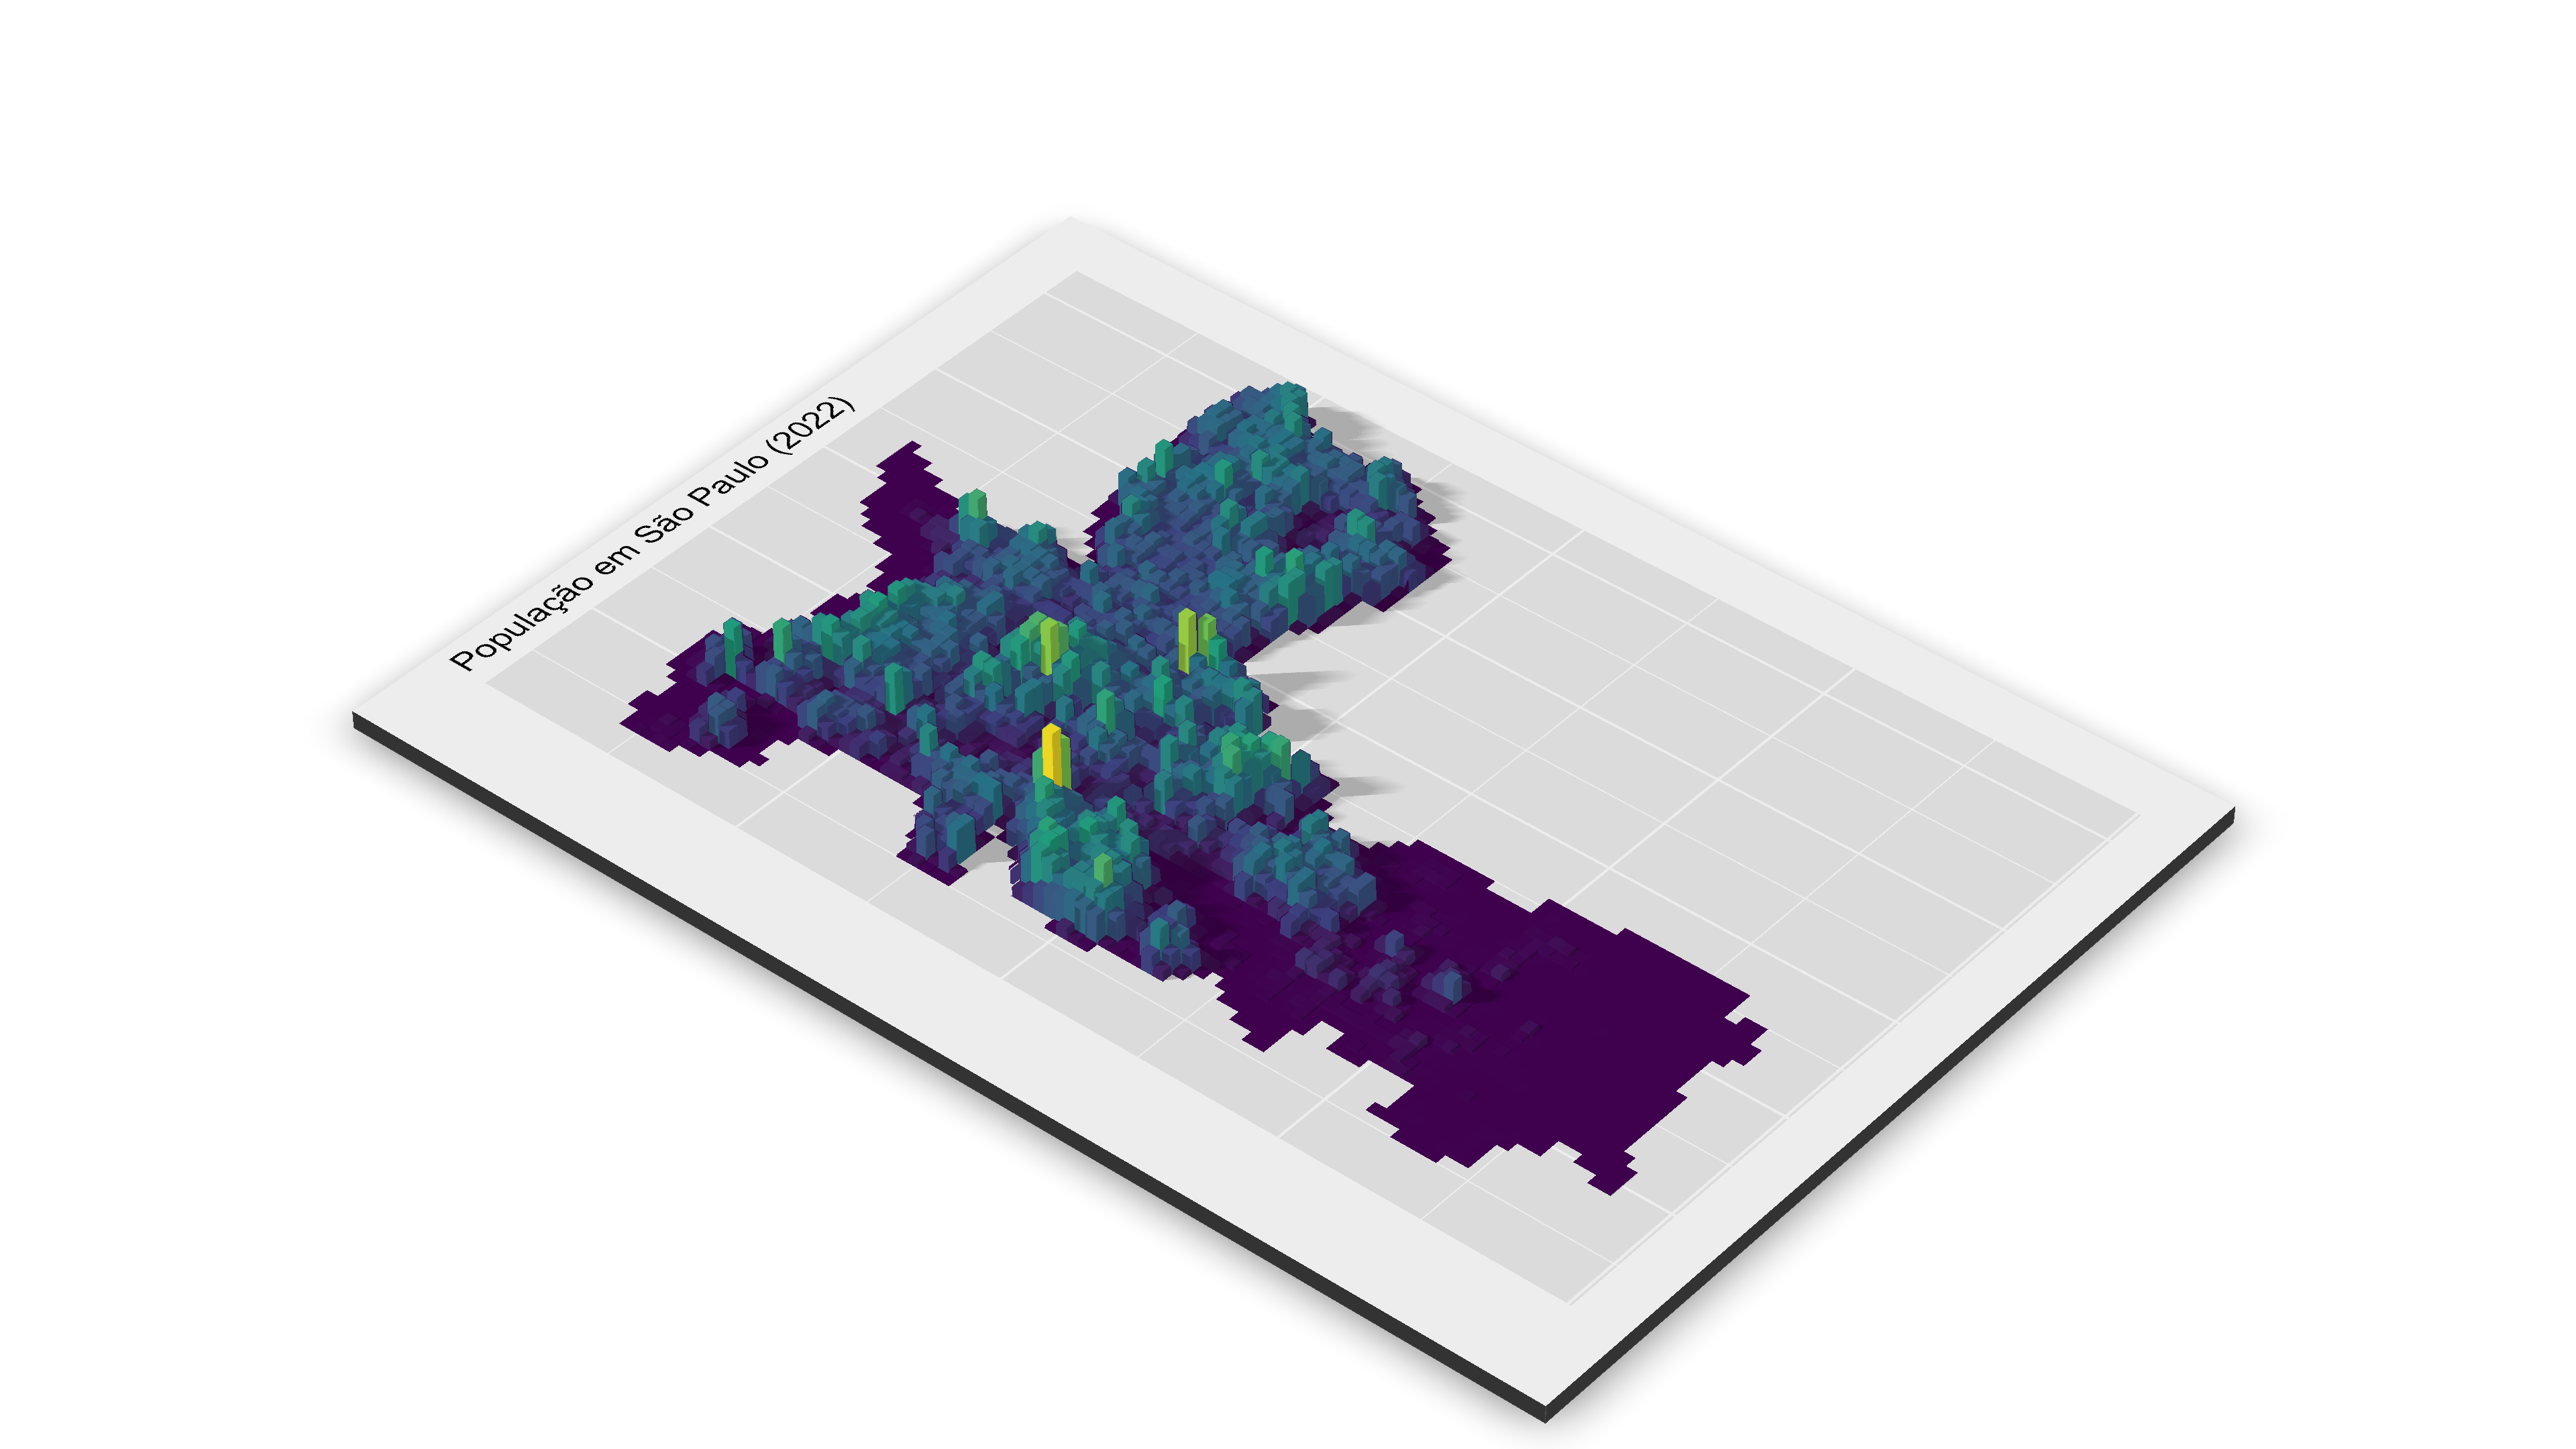
\includegraphics[width = \paperwidth, height = \paperheight]{imagens/mapa3d.png}
    \end{figure}
\end{frame}

\frame{\titlepage}

% \begin{frame}
% \frametitle{Sumário}
% \tableofcontents
% \end{frame}

\section{Introdução}

\begin{frame}
    \frametitle{Por que cidades existem?}
    \begin{quote}
        City life constantly attracts newcomers, and the trade-mark of newcomers is bringing \textcolor{DarkGreen}{``new ways of looking at things, and maybe new ways of solving old problems''}. Newcomers are strangers to the city, and things that the old, well settled residents stopped noticing because of their familiarity, seem bizarre and call for explanation when seen through the eye of a stranger. For strangers, and particularly for the newcomers among them, nothing in the city is `natural'; nothing is taken for granted by them. \textcolor{DarkBlue}{Newcomers are born and sworn enemies of tranquillity and self-congratulation. This is not perhaps a situation to be enjoyed by the city natives --- but this is also their good luck}. City is at its best, most exuberant and most lavish in offered opportunities, when its ways and means are challenged, questioned, and put on the defendants' bench

        \raggedleft{\cite{bauman2003city}}
    \end{quote}
\end{frame}

\begin{frame}
    \frametitle{Motivação econômica \cite{brueckner2011lectures}}
    \begin{itemize}
        \item<1-> Aglomeração Tecnológica
        \begin{itemize}
            \item<1> \textcolor{DarkBlue}{Aumento de produtividade} dos trabalhadores, na medida em que os empregos são mais concentrados e há \textcolor{DarkBlue}{``transbordamento'' de conhecimento} entre as firmas da região
            \item<1> Uma oferta maior e mais diversa de trabalho causa \textcolor{DarkBlue}{maior competitividade e eficiência} na escolha da pessoa certa para cada cargo
        \end{itemize}
        \item<2-> Aglomeração Pecuniária
        \begin{itemize}
            \item<2> \textcolor{DarkBlue}{Reduz os custos das firmas}, sem alterar sua produtividade
            \item<2> Com maior demanda por serviços como segurança, limpeza, contratação e advocacia, estes mercados se desenvolvem, tornam-se mais competitivos, eficientes e baratos
        \end{itemize}
        \item<3-> Aglomeração de Varejo
        \begin{itemize}
            \item<3> O consumidor pode escolher entre mais opções e se desloca menos entre seus destinos caso queria comprar mais de um item
            \item<3> Os comerciantes ganham também, visto que com mais consumidores e maior fluxo, maiores as vendas
        \end{itemize}
        \item<4-> Custo de Transporte
        \begin{itemize}
            \item<4> A redução do custo de transporte, que pode ser considerada uma economia de aglomeração pecuniária, acontece não apenas para os trabalhadores, que se deslocam menos às oportunidades de emprego, mas também às firmas que gastam menos transportando seus bens e serviços
        \end{itemize}
    \end{itemize}

\end{frame}


\begin{frame}
    \frametitle{O problema do custo social}
    \begin{columns}[T]
        \column{.5\textwidth}
        \cite{bauman2003city}

        Newcomers are born and sworn enemies of tranquillity and self-congratulation. This is not perhaps a situation to be enjoyed by the city natives --- but this is also their good luck.

        \column{.5\textwidth}
        \cite{coase2013problem}

        The question is commonly thought of as one in which A inflicts harm on B and what has to be decided is: how should we restrain A? But this is wrong. \textcolor{DarkBlue}{We are dealing with a problem of a reciprocal nature}. To avoid the harm to B would inflict harm on A. The real question that has to be decided is: should A be allowed to harm B or should B be allowed to harm A?     

    \end{columns}
\end{frame}

\begin{frame}
    \frametitle{O problema do custo social}

    \begin{quote}
        ``Cities should replace the current lengthy and uncertain permitting process with a simple system of fees. If tall heights create costs by blocking light or views, then form a reasonable estimate of those costs and charge the builder appropriately. If certain activities are noxious to neighbors, then we should estimate the social costs and charge builders for them, just as we should charge drivers for the costs of their congestion. Those taxes could then be given to the people who are suffering, such as the neighbors who lose light from a new construction project.''

        \raggedleft{\cite{glaeser2011triumph}}
    \end{quote}

    \begin{itemize}
        \item<2> Simplificar regras, diminuir incertezas e diminuir burocracia
        \item<2> Taxar atividades nocivas e utilizar o dinheiro para compensar a parte prejudicada
    \end{itemize}
    
\end{frame}

\begin{frame}
    \frametitle{Regulação em São Paulo}

    Os mecanismos de regulação são principalmente definidos pelo atual Plano Diretor Estratégico \cite[PDE]{PDE}

    \begin{itemize}
        \item Entre os 17 objetivos estabelecidos, ao menos nove estão relacionados a estratégias de adensamento urbano \cite{lima2021alem}
        \item Dispositivos para imóveis já existentes e para novos empreendimentos
        \item Principais instrumentos: CA, cota-parte e gabarito
        \item Regulação incentiva adensamento em áreas mais desejáveis (no entorno de serviços públicos, trabalho, transporte público de alta capacidade, etc.)
    \end{itemize}
\end{frame}

\begin{frame}
    \frametitle{O problema}
    \centering

    Estes instrumentos de regulação são capazes de determinar a densidade populacional?

\end{frame}

\section{Teoria}

\begin{frame}
    \frametitle{Construção do modelo econômico}
    \framesubtitle{\cite{papageorgiou2012essay, fujita1989urban,brueckner2011lectures}}

    \begin{columns}
        \column{.5\textwidth}
        \begin{itemize}
            \item Pessoas querem moradias e consumir bens
            \begin{itemize}
                \item Quanto mais perto do trabalho moram, menos é gasto com transporte
                \item Com mais demanda pelas regiões centrais, mais caro fica o $m^2$
            \end{itemize}
            \item Imobiliárias querem maximizar seus lucros
            \begin{itemize}
                \item Prefere construir onde há um $m^2$ mais caro
                \item Vale a pena construir mais pavimentos onde o custo marginal de verticalizar é igual ao custo marginal da terra
            \end{itemize}
            \item Resultado: A densidade aumenta na medida em que a distância ao centro diminui
        \end{itemize}

        \column{.5\textwidth}
        \begin{tikzpicture}

    \begin{axis}[standard,
        xtick={0},
        ytick={0},
        xticklabels = {},
        yticklabels = {},
        samples=100,
        xlabel={Distância ao centro ($x$)},
        ylabel={\$},
        xmin=0,xmax=2,
        ymin=0,ymax=1,
        y label style={anchor=east},
        x label style={anchor=north},
    ]
    
\addplot[name path=F,domain={0:2}]{e^(-x)} node[pos=1] (point) {};
\node [right] at (point) {$p$};



    
\end{axis}
\end{tikzpicture}
    \end{columns}
\end{frame}

\begin{frame}
    \frametitle{Introdução de novos componentes}
    \framesubtitle{\cite{papageorgiou2012essay, fujita1989urban,brueckner2011lectures}}

    \begin{columns}
        \column{.5\textwidth}
        \begin{tikzpicture}

    \begin{axis}[standard,
        xtick={0},
        ytick={0},
        xticklabels = {},
        yticklabels = {},
        samples=100,
        xlabel={Distância ao centro ($x$)},
        ylabel={\$},
        xmin=0,xmax=2,
        ymin=0,ymax=1,
        y label style={anchor=east},
        x label style={anchor=north},
    ]
    
\addplot[name path=F,domain={0:2}]{e^(-x)} node[pos=1] (point) {};
\node [right] at (point) {$p$};



    
\end{axis}
\end{tikzpicture}

        \column{.5\textwidth}
        \begin{tikzpicture}

    \begin{axis}[standard,
        xtick={0},
        ytick={0},
        xticklabels = {},
        yticklabels = {},
        samples=100,
        xlabel={Distância ao centro ($x$)},
        ylabel={\$},
        xmin=0,xmax=2,
        ymin=0,ymax=1,
        y label style={anchor=east},
        x label style={anchor=north},
    ]
    
\addplot[name path=F,domain={0:2}]{e^(-x)} node[pos=1] (point1) {};
\node [right] at (point1) {$p_R$};

\addplot[name path=G,domain={0:2}]{0.5 * e^(-0.5*x) + .1} node[pos=1] (point2) {};
\node [right] at (point2) {$p_P$};

\path [name intersections={of=G and F, by = intersec}]; 
\draw[dashed] (intersec) -- (intersec|-{axis cs:0,0});

    
\end{axis}
\end{tikzpicture}
    \end{columns}
\end{frame}

% \begin{frame}
%     \frametitle{Implicações em policy}
% \end{frame}


\section{Dados}

% \begin{frame}
%     \frametitle{Sumário}
%     \begin{columns}
%         \column{.5\textwidth}
%         \tableofcontents[currentsection]

%         \column{.5\textwidth}
%         \begin{enumerate}
%             \item Dados do Censo
%             \item Dados do IPTU
%             \item Cruzamento dos dados
%             \item Resultados preliminares
%         \end{enumerate}
%     \end{columns}
    
% \end{frame}

\begin{frame}
    \frametitle{Dados do Censo}
    \begin{columns}
        \column{.4\textwidth}
        \begin{figure}
            \centering
            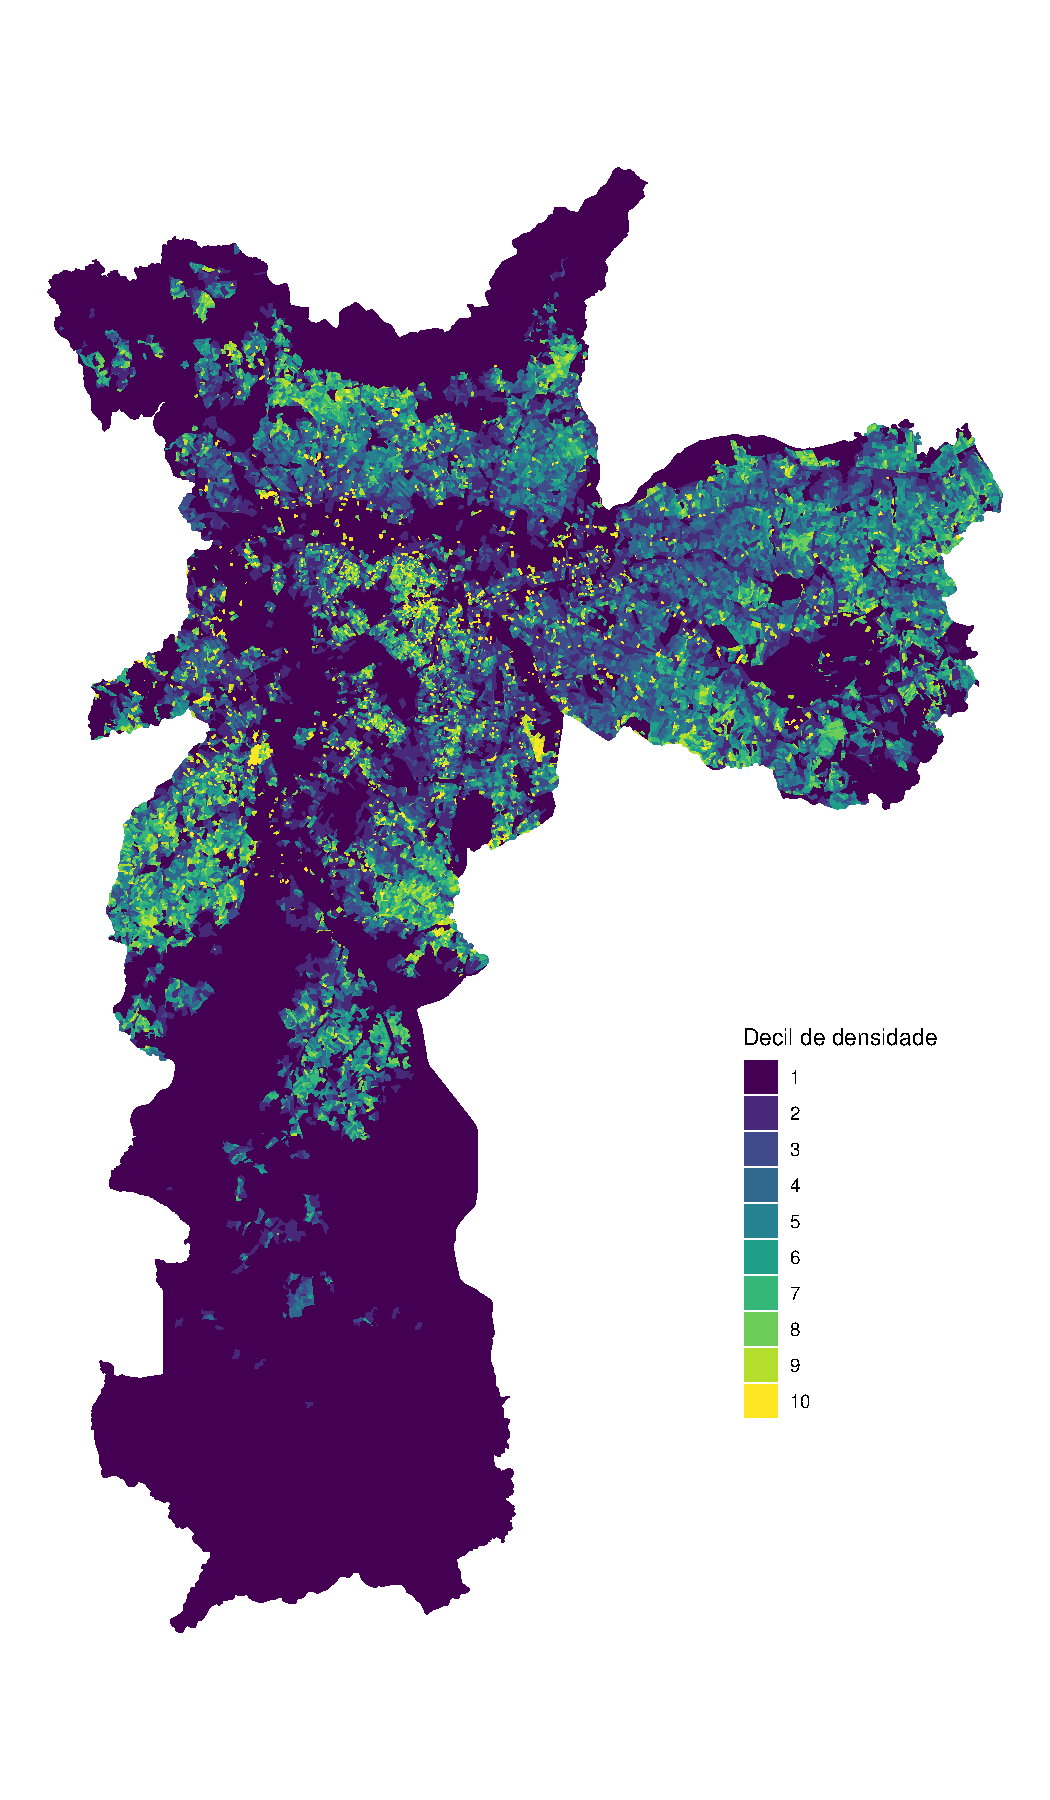
\includegraphics[height=.95\textheight]{imagens/mapa.pdf}
        \end{figure}

        \column{.6\textwidth}
        \begin{itemize}
            \item Dados preliminares do Censo de 2022
            \item Nível da observação: setor censitário
            \item 11.451.999 de habitantes e 4.996.529 de domicílios, dos quais 4.316.336 estão ocupados
        \end{itemize}
        \begin{figure}
            \centering
            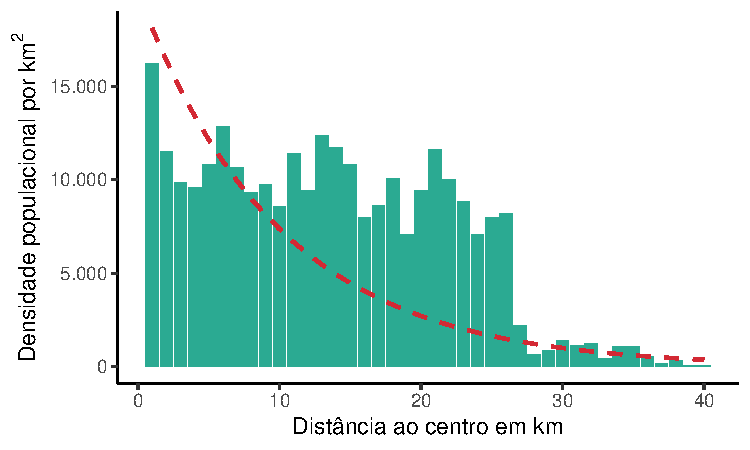
\includegraphics[width = .7\textwidth]{imagens/densidade_distcentro.pdf}
        \end{figure}
    \end{columns}
\end{frame}



\begin{frame}
    \frametitle{Cálculo dos indicadores}
    \bigskip

    \begin{columns}[T]
        \column{.33\textwidth} 
        \centering
        \textbf{Coeficiente de Aproveitamento}
        
        \begin{equation*}
            CA=\frac{\textit{Área Construída}}{\textit{Área do Terreno}}
        \end{equation*}

        \column{.33\textwidth} 
        \centering
        \textbf{Cota Parte}

        \begin{equation*}
            CP=\frac{\textit{Área do Terreno}}{\textit{Número de Unidades}}
        \end{equation*}

        \column{.33\textwidth}
        \centering 
        \textbf{Verticalização}

        \begin{equation*}
            \textit{Pavimentos (?)}
        \end{equation*}
    \end{columns}

    \bigskip

    \begin{figure}
        \centering
        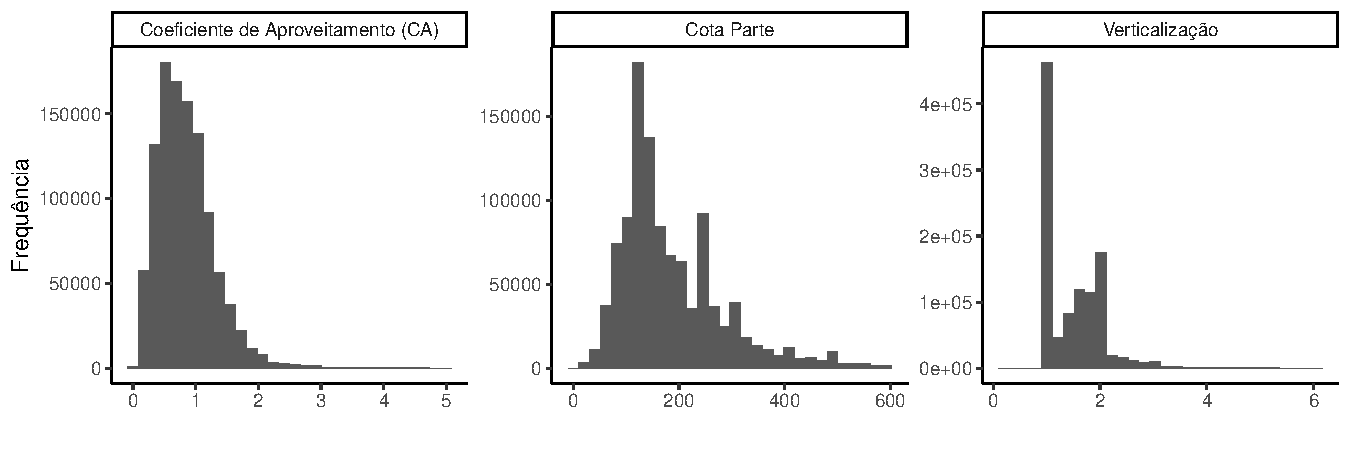
\includegraphics[width = .85\textwidth]{imagens/indicadores.pdf}
    \end{figure}
\end{frame}


\begin{frame}
    \frametitle{Verticalização}
    \begin{figure}
        \centering
        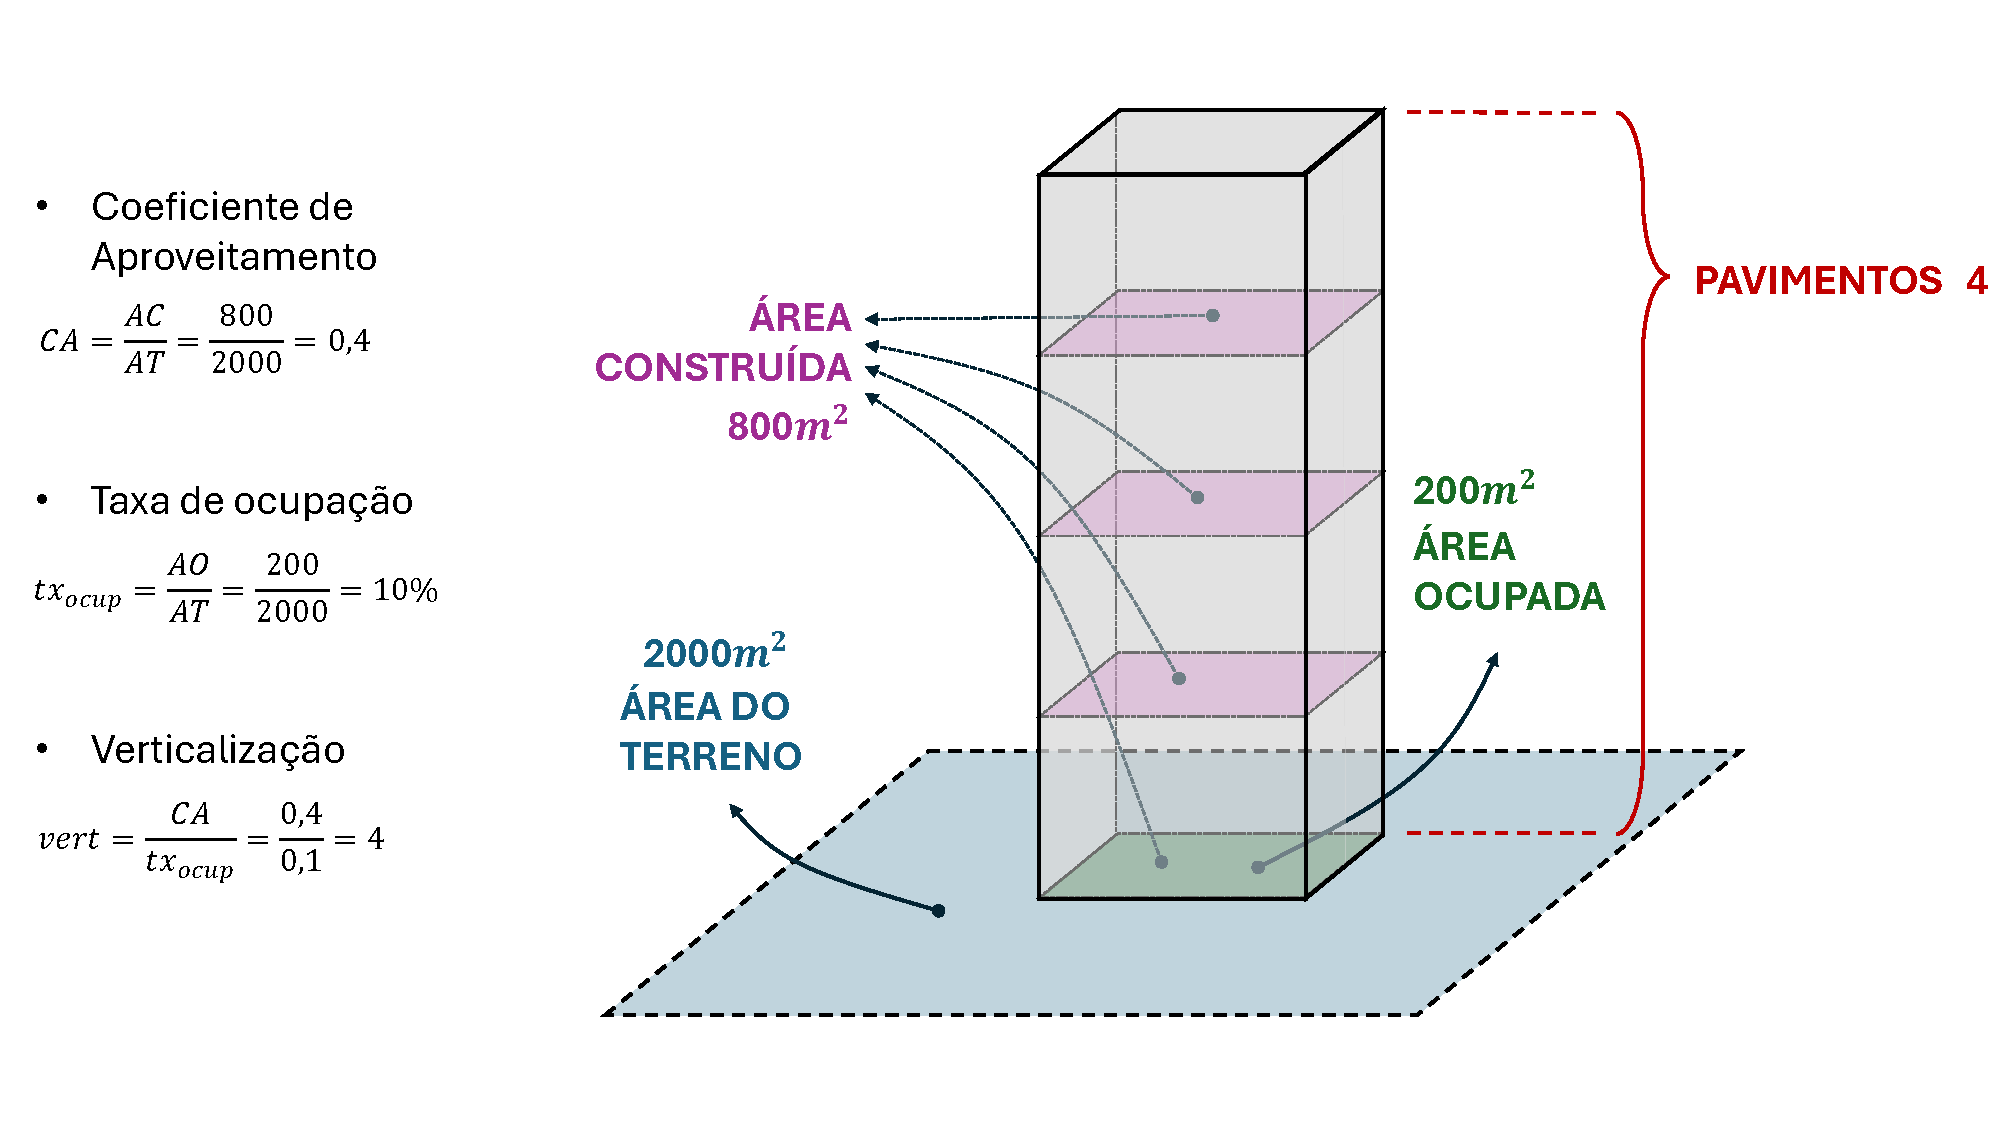
\includegraphics[height = .9\textheight]{imagens/desenho.pdf}
    \end{figure}
\end{frame}


\begin{frame}
    \frametitle{Verticalização}
    \begin{equation*}
        \text{Pavimentos}=\frac{\text{AC}}{\text{AO}}=\frac{\text{AC}}{\text{AT}\cdot\underbrace{\frac{\text{AO}}{\text{AT}}}_\text{tx\_ocup}}=\frac{\text{AC}}{\text{AT}}\div\frac{\text{AO}}{\text{AT}}=\frac{\text{CA}}{\text{tx\_ocup}}
    \end{equation*}
    \begin{figure}
        \centering
        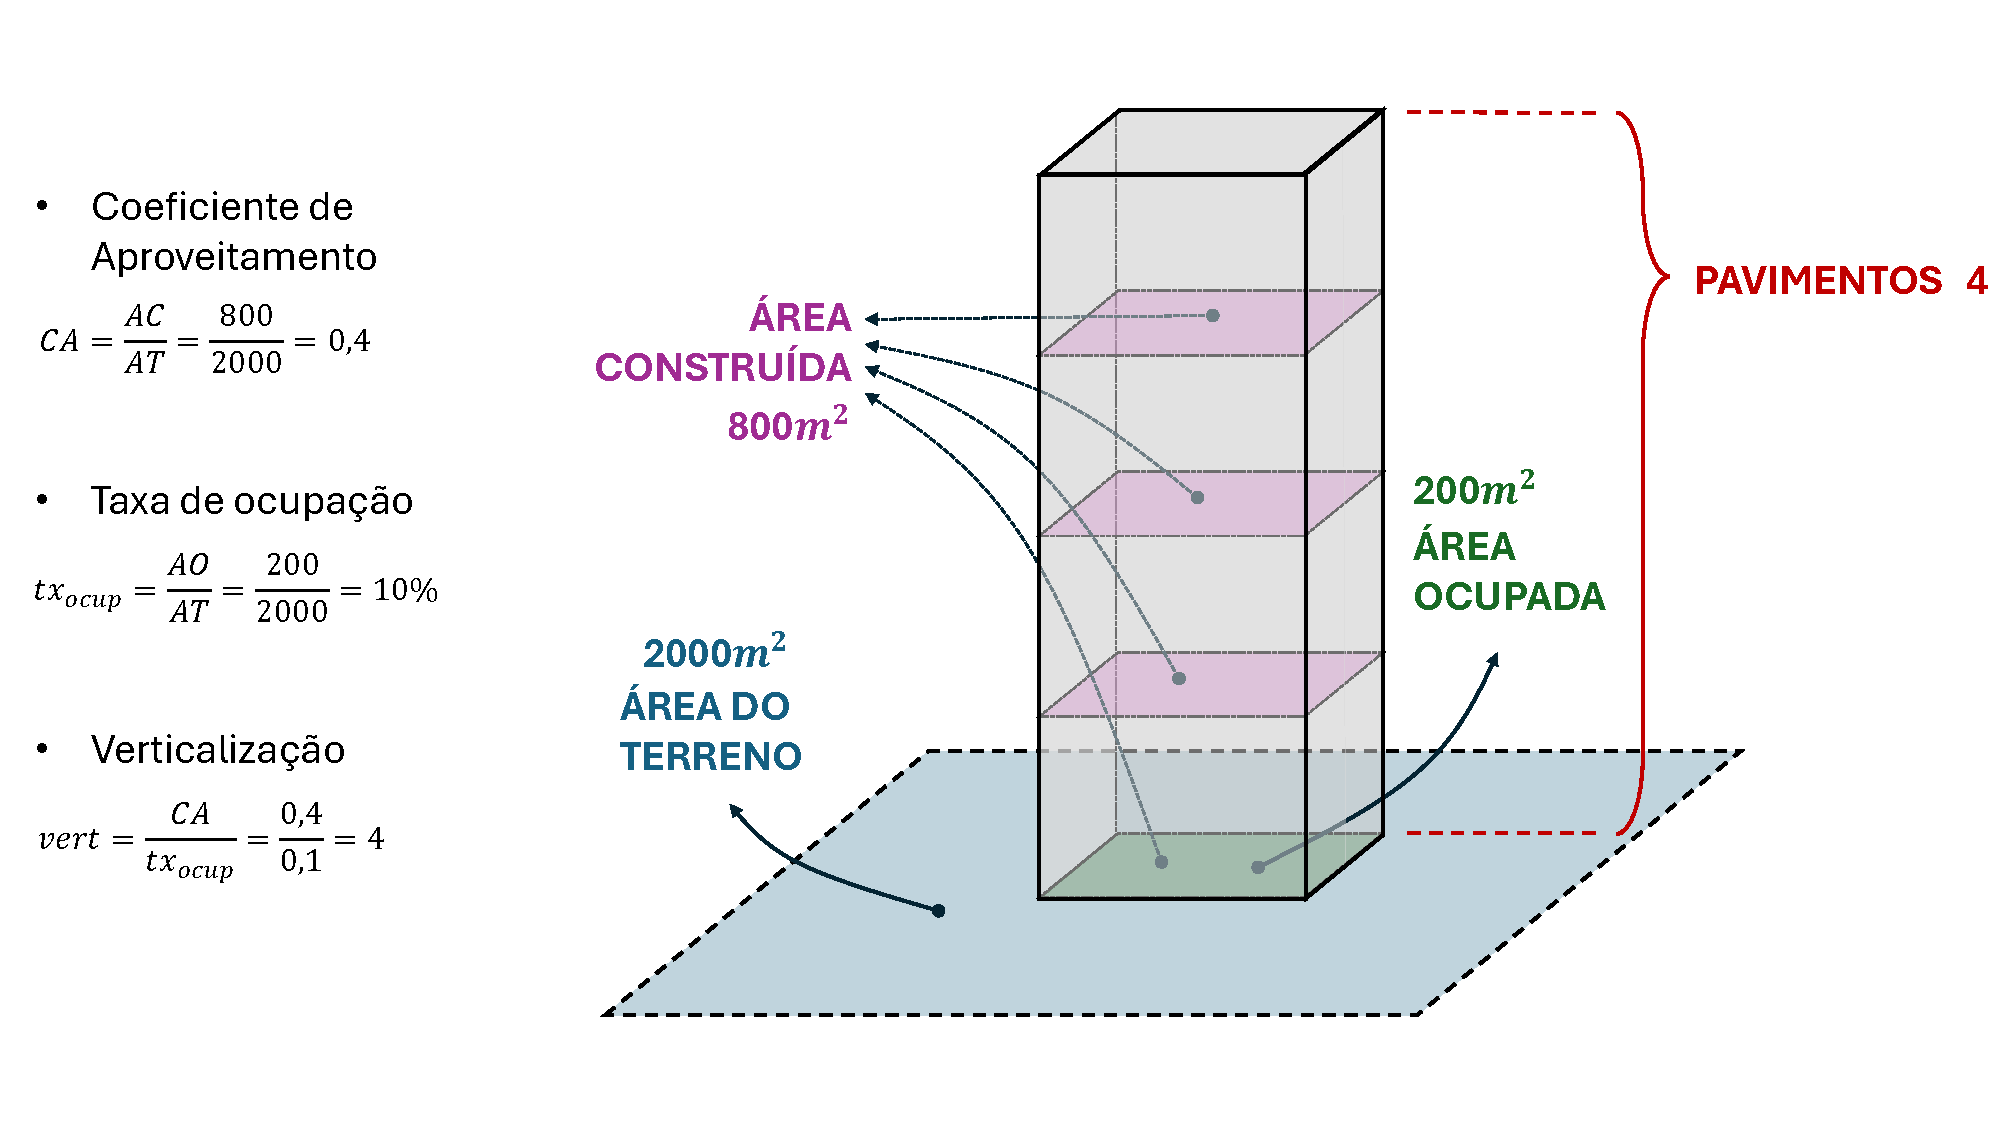
\includegraphics[height = .6\textheight]{imagens/desenho.pdf}
    \end{figure}
\end{frame}

\begin{frame}
    \frametitle{Área construída em São Paulo}
    \begin{figure}
        \centering
        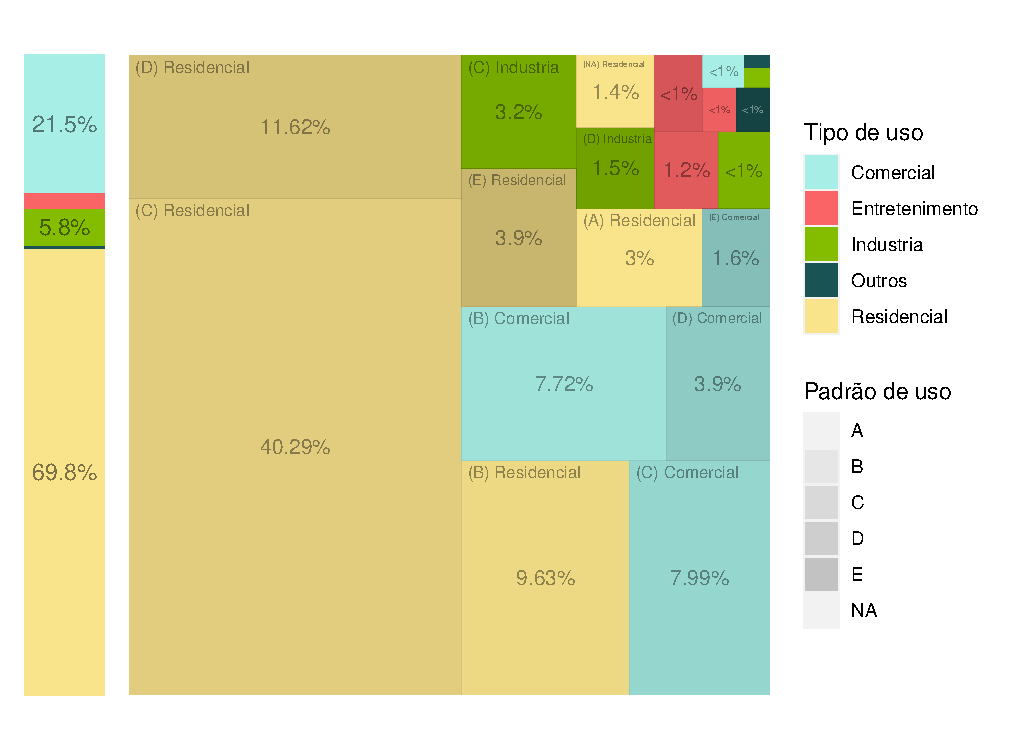
\includegraphics[height = .95\textheight]{imagens/tree_area_construida.pdf}
    \end{figure}
\end{frame}

\begin{frame}
    \frametitle{Dados do IPTU}
    \begin{columns}
        \column{.5\textwidth}
        \begin{figure}
            \centering
            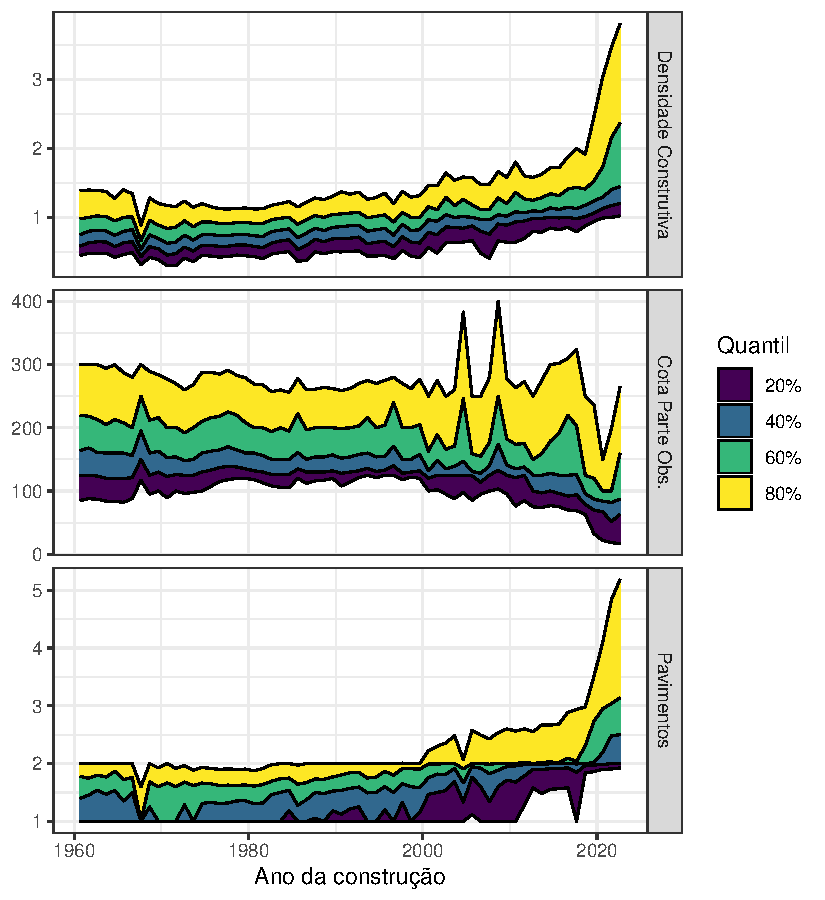
\includegraphics[height = .9\textheight]{imagens/indicadores_tempo_small.pdf}
        \end{figure}

        \column{.5\textwidth}
        \begin{itemize}
            \item Estoque (e não fluxo) imobiliário.
            \item Estão cadastrados 3.096.719 contribuintes, dos quais \textcolor{BrickRed}{2.641.635} são habitacionais
        \end{itemize}

        \begin{figure}
            \centering
            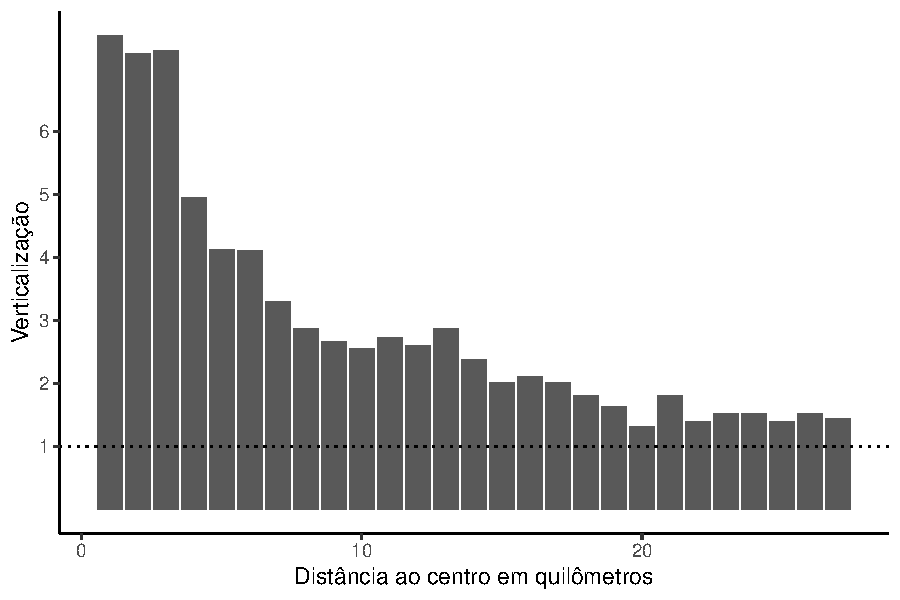
\includegraphics[width = .8\textwidth]{imagens/verticalizacao.pdf}
        \end{figure}
    \end{columns}
    
\end{frame}

\begin{frame}
    \frametitle{Cruzamento dos dados}
    \framesubtitle{Abordagem de join geográfico}

    \begin{figure}
        \centering
        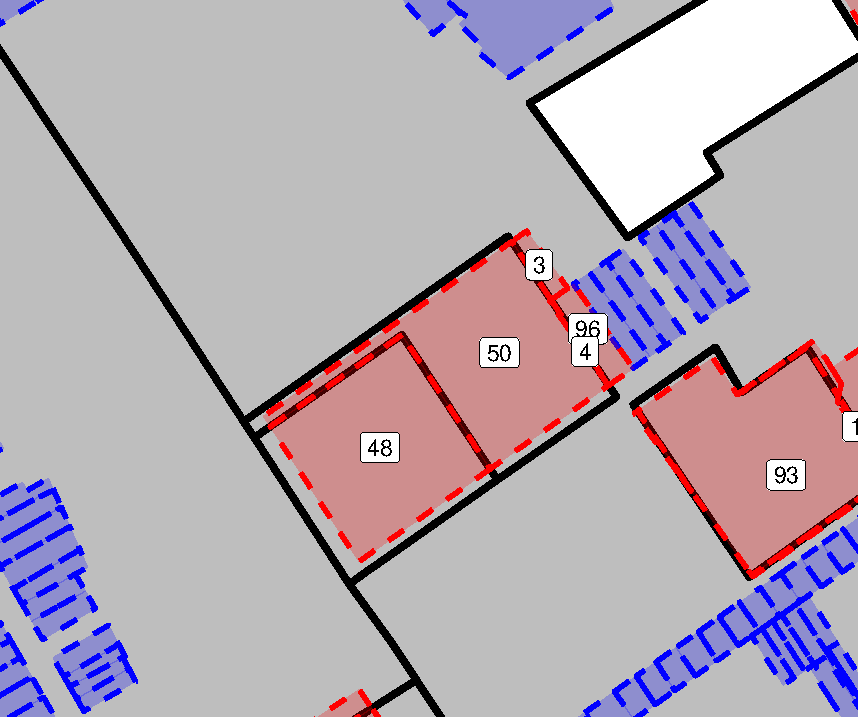
\includegraphics[width = .6\linewidth]{imagens/corte_lote.pdf}
    \end{figure}
\end{frame}

\begin{frame}
    \frametitle{Cruzamento dos dados}
    \framesubtitle{Abordagem de raster}

    \begin{figure}
        \centering
        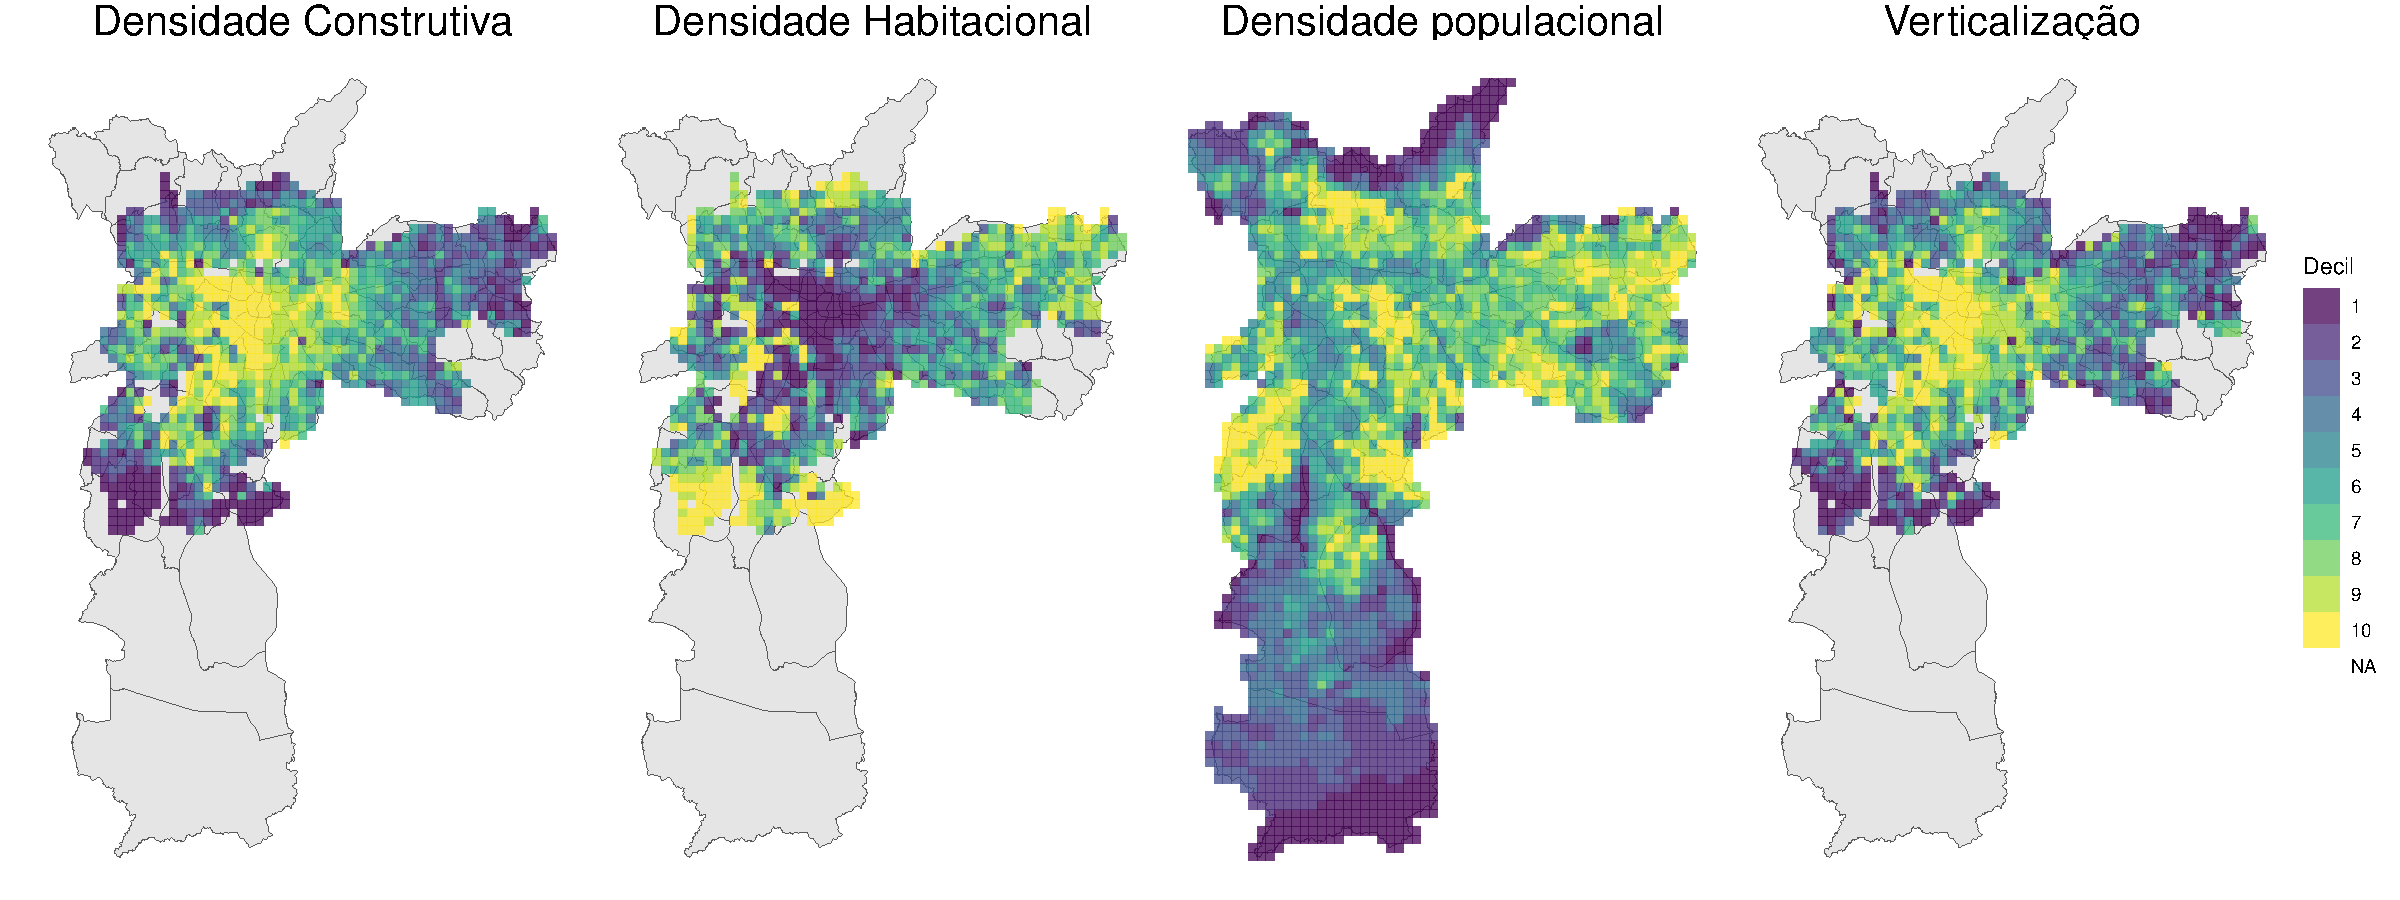
\includegraphics[width = \linewidth]{imagens/rasters_wide.pdf}
    \end{figure}
\end{frame}

\begin{frame}
    \frametitle{Problemas no join}
    \begin{columns}[T]
        \column{.5\textwidth}
        \textbf{Definição domicílio}
        % \rule{\textwidth}{.1pt}
        \smallskip

        \begin{itemize}
            \item Separado: limitado por paredes e coberto por um teto com a finalidade de dormir, preparar, consumir seus alimentos e proteger-se do meio ambiente
            \item Independente: entrada e saída sem passar por locais de moradias de outras pessoas
        \end{itemize}

        \column{.5\textwidth}
        \textbf{Definição de unidade}
        % \rule{\textwidth}{.1pt}
        \smallskip

        ``A cada imóvel urbano corresponderá um número de inscrição no Cadastro Imobiliário Fiscal, entendendo-se como imóvel: I - a área de terreno, construído ou não, definida em matrícula do competente Serviço de Registro de Imóveis ou em transcrições ainda vigente''
    \end{columns}

    \begin{figure}
        \centering
        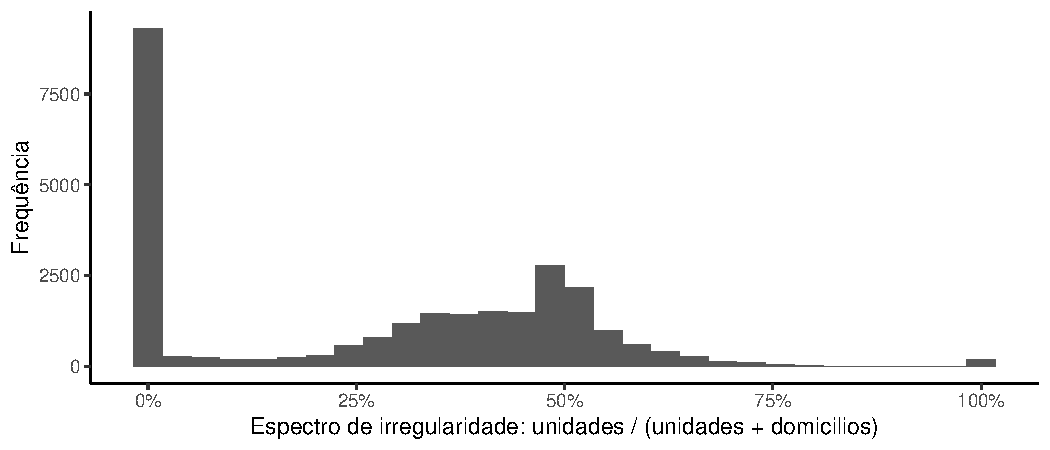
\includegraphics[width = .7\textwidth]{imagens/disparidade_censoIPTU.pdf}
    \end{figure}
\end{frame}

\begin{frame}
    \frametitle{Problemas no join}

    \begin{columns}[T]
        \column{.5\linewidth}
        \begin{figure}
            \centering
            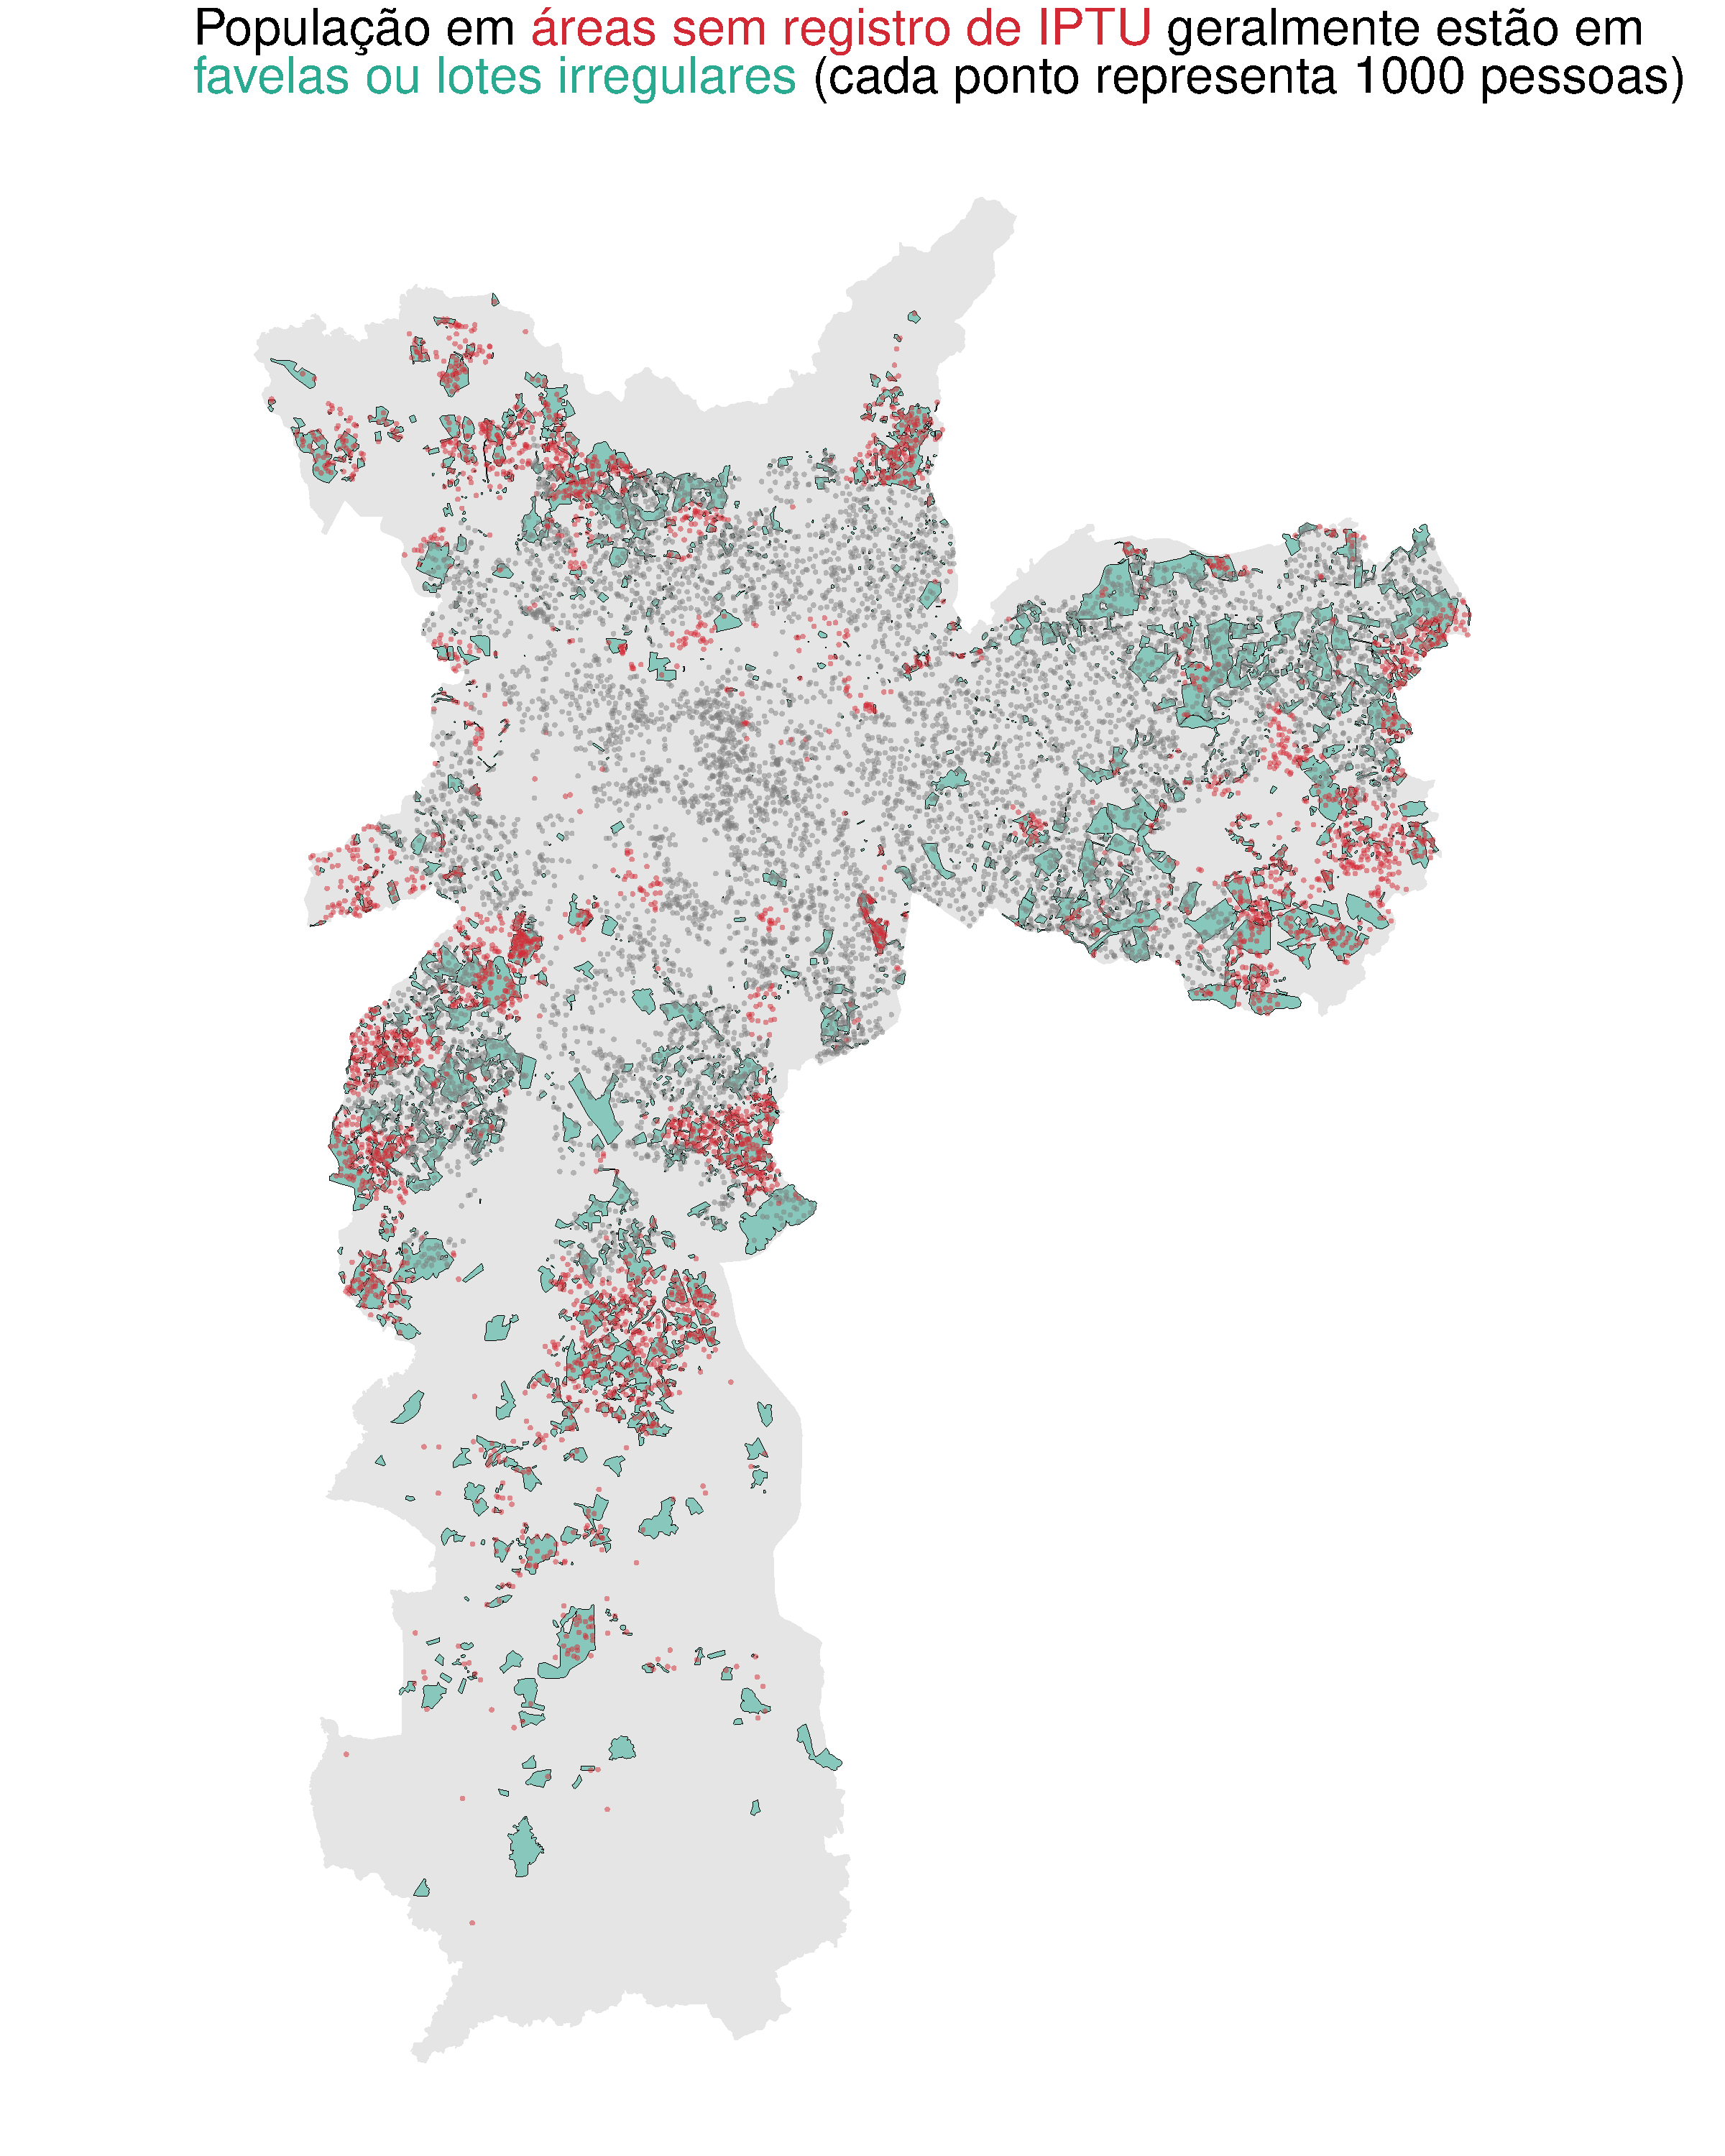
\includegraphics[width = 1\linewidth]{imagens/mapa_pontos.pdf}
        \end{figure}

        \column{.5\linewidth}
        \begin{figure}
            \centering
            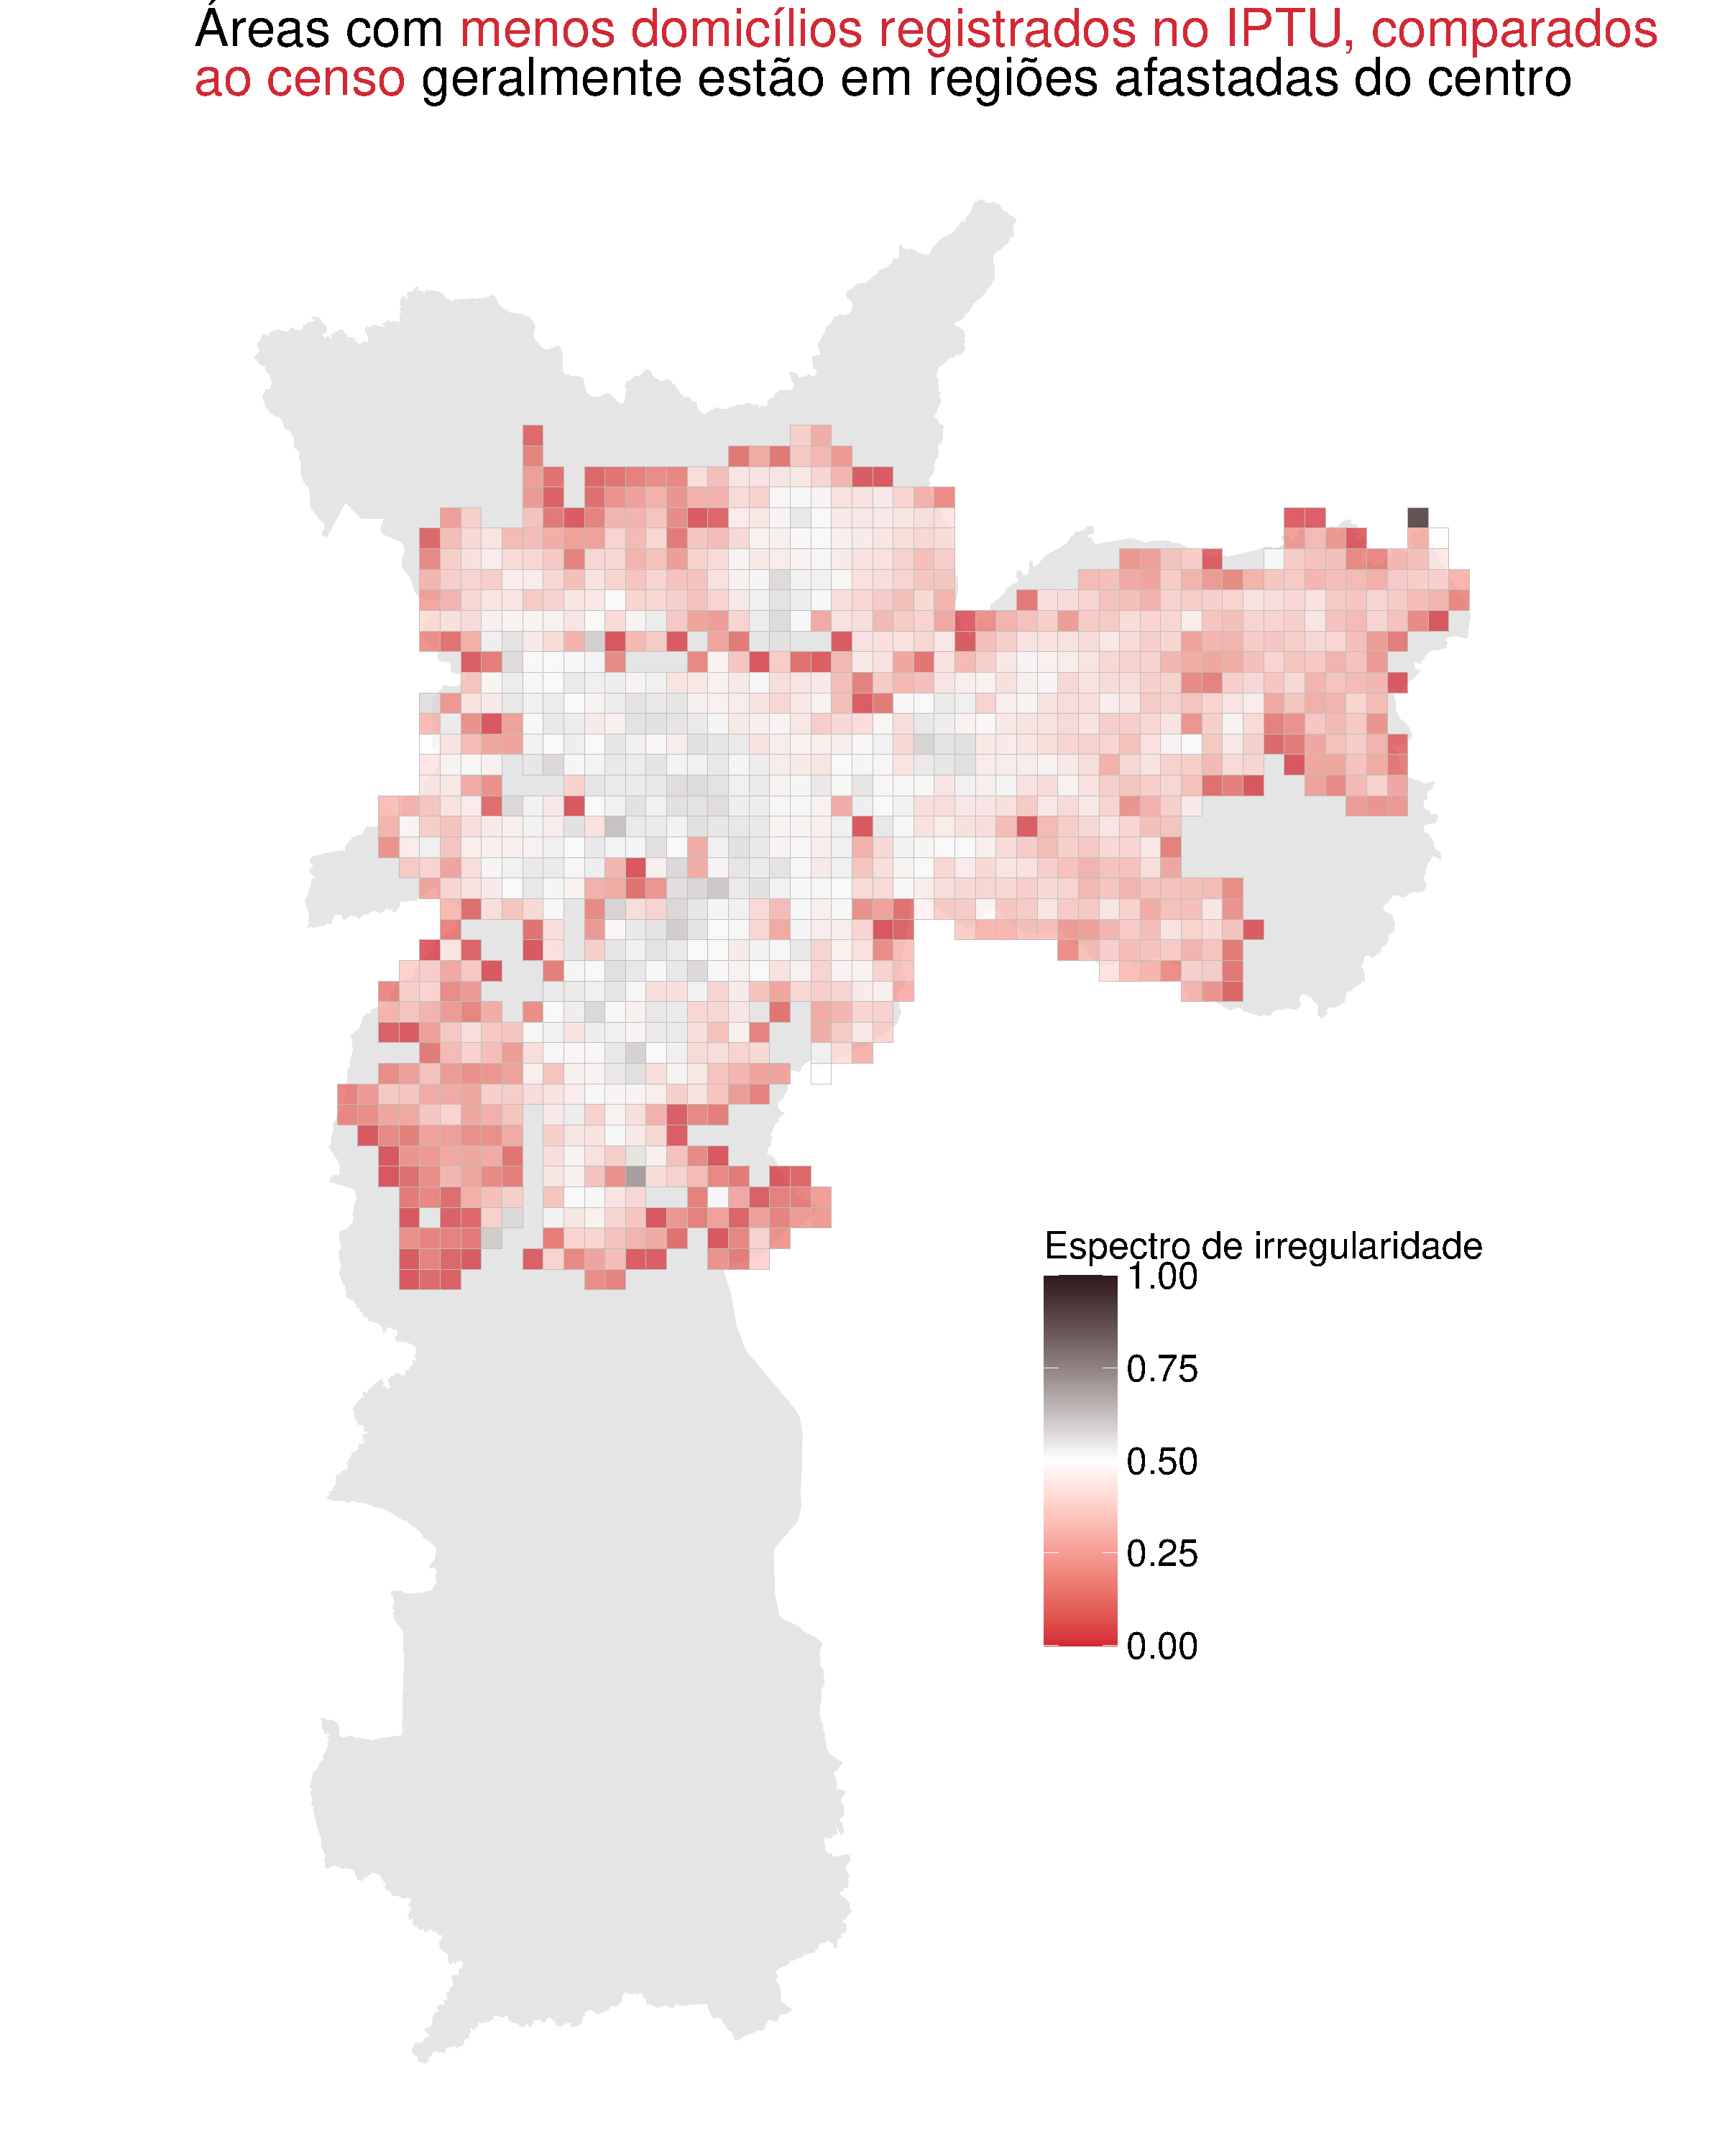
\includegraphics[width = \linewidth]{imagens/balanco_raster.pdf}
        \end{figure}
    \end{columns}
\end{frame}

\begin{frame}
    \frametitle{Áreas mais densas de São Paulo}

    \begin{table}
        \fontsize{4pt}{10}
        \caption{Células do \textit{raster} que apresentam a maior densidade populacional}
        \begingroup
\fontsize{6.8pt}{8.1pt}\selectfont
\begin{longtable}{lrrrrr}
\toprule
 & \multicolumn{4}{c}{Favelas} &  \\ 
\cmidrule(lr){2-5}
Variável & 1. Paraisópolis & 2. Heliópolis  & 4. Paraisópolis & 5. Heliópolis & 3. Sé (Bela Vista) \\ 
\midrule\addlinespace[2.5pt]
População & 29.598 & 25.280 & 23.824 & 22.920 & 24.576 \\ 
Domicílios (Censo) & 11.655 & 10.178 & 9.361 & 9.001 & 17.875 \\ 
Unidades (IPTU) & 0 & 1.857 & 7 & 3 & 21.057 \\ 
Espectro irregularidade & 0.00\% & 15.43\% & 0.08\% & 0.03\% & 54.09\% \\ 
Densidade habitacional & 46.247 & 39.500 & 37.225 & 35.813 & 38.400 \\ 
Área & 640.000 & 640.000 & 640.000 & 640.000 & 640.000 \\ 
\bottomrule
\end{longtable}
\endgroup


        \addtocounter{table}{-1}
    \end{table}

    Densidade média em São Paulo: 7.529 $hab/km^2$
\end{frame}

\section{Análise}

\begin{frame}
    \frametitle{Construção do modelo empírico}
    \fontsize{12pt}{7}
    \begin{equation*}
        \textit{densidade}_i = \beta_0 + \beta_1 \cdot \textit{CA}_i + \beta_2 \cdot\textit{cota parte}_i + \beta_3\cdot\textit{verticalização}_i + \varepsilon_i
        \label{eq:reg}
    \end{equation*}
\end{frame}

\begin{frame}
    \frametitle{Nível da observação - Problema do setor censitário}
    \begin{columns}
        \column{.5\textwidth}
        \begin{figure}
            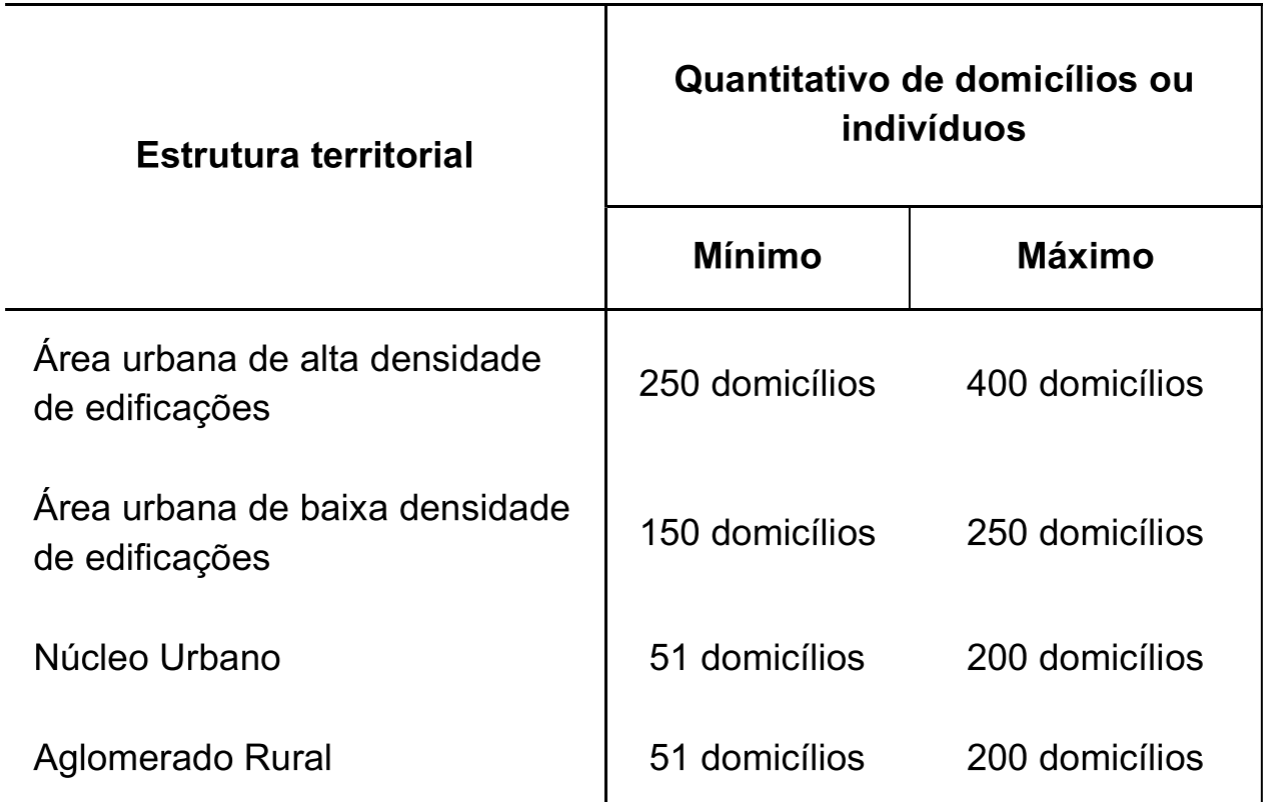
\includegraphics[width = \textwidth]{imagens/tabela_ibge.png}
        \end{figure}


        \column{.5\textwidth}
        \textbf{Fatores levados em consideração}
        \begin{itemize}
            \item Elementos na paisagem que se constituam em barreiras naturais ou artificiais, e, assim, dificultam o percurso do setor, levando ao aumento do tempo de coleta
            \item Pontos de referência estáveis e de fácil identificação
            \item Limites de estruturas territoriais (bairros, quadras, etc.)
        \end{itemize}

    \end{columns}
\end{frame}

\begin{frame}
    \frametitle{Resultados}
    \begin{table}
        \caption{Regressão para densidade populacional}
        \begingroup
\fontsize{9.0pt}{10.8pt}\selectfont
\begin{longtable}{lrlrlrlrl}
\toprule
 & \multicolumn{4}{c}{Espectro irregularidade: 35 a 65\%} & \multicolumn{4}{c}{Espectro irregularidade: 45 a 55\%} \\ 
\cmidrule(lr){2-5} \cmidrule(lr){6-9}
 & \multicolumn{2}{c}{Nível (A)    } & \multicolumn{2}{c}{Log (B)    } & \multicolumn{2}{c}{Nível (C)    } & \multicolumn{2}{c}{Log (D)    } \\ 
\cmidrule(lr){2-3} \cmidrule(lr){4-5} \cmidrule(lr){6-7} \cmidrule(lr){8-9}
  & Coeficiente & * & Coeficiente  & *  & Coeficiente   & *   & Coeficiente    & *    \\ 
\midrule\addlinespace[2.5pt]
(Intercept) & 11876.195 & *** & 9.993 & *** & 4258.148 & * & 9.671 & *** \\ 
cota\_parte & -9.892 & *** & -0.002 & *** & -9.410 & ** & -0.002 & *** \\ 
verticalizacao & 816.466 & . & 0.014 &  & 1398.701 & ** & 0.024 & . \\ 
CA & 10951.872 & *** & 0.197 & *** & 11470.672 & *** & 0.274 & *** \\ 
{R2} & {0.507} & {} & {0.638} & {} & {0.639} & {} & {0.737} & {} \\ 
R2 ajustado & 0.505 &  & 0.636 &  & 0.636 &  & 0.735 &  \\ 
Observações & 741 &  & 741 &  & 332 &  & 332 &  \\ 
\bottomrule
\end{longtable}
\endgroup


    \end{table}
\end{frame}

\begin{frame}
    \frametitle{Problemas do modelo: Violação das suposições de Gauss-Markov}

    \begin{enumerate}
        \item Forma funcional

        \begin{align*}
            &\textit{densidade}_i 
            &=\beta_0 
            &+\beta_1 (\textit{CA}_i) 
            &+\beta_2 (\textit{cota parte}_i)
            &+\beta_3 (\textit{verticalização}_i)
            &+\varepsilon_i \\
            &\frac{\textit{População}_i}{\textit{A. Total}_i}
            &=\beta_0
            &+\beta_1\left(\frac{\textit{A. Construída}_i}{\textit{A. do Terreno}_i}\right)
            &+\beta_2\left(\frac{\textit{A. Terreno}_i}{\textit{N. unidades}_i}\right)
            &+\beta_3\left(\frac{\textit{A. Construída}_i}{\textit{A. Ocupada}_i}\right)
            &+\varepsilon_i
        \end{align*}

        \bigskip
        \item<2-> Omissão de regressores relevantes
        \begin{itemize}
            \item $H_0:$ Indicadores \textbf{são} eficientes para definir a densidade
            \item $H_A:$ Indicadores \textbf{não são} eficientes para definir a densidade
        \end{itemize}    
    \end{enumerate}
\end{frame}

\begin{frame}
    \frametitle{Construção da \textit{random forest}}
    \begin{figure}
        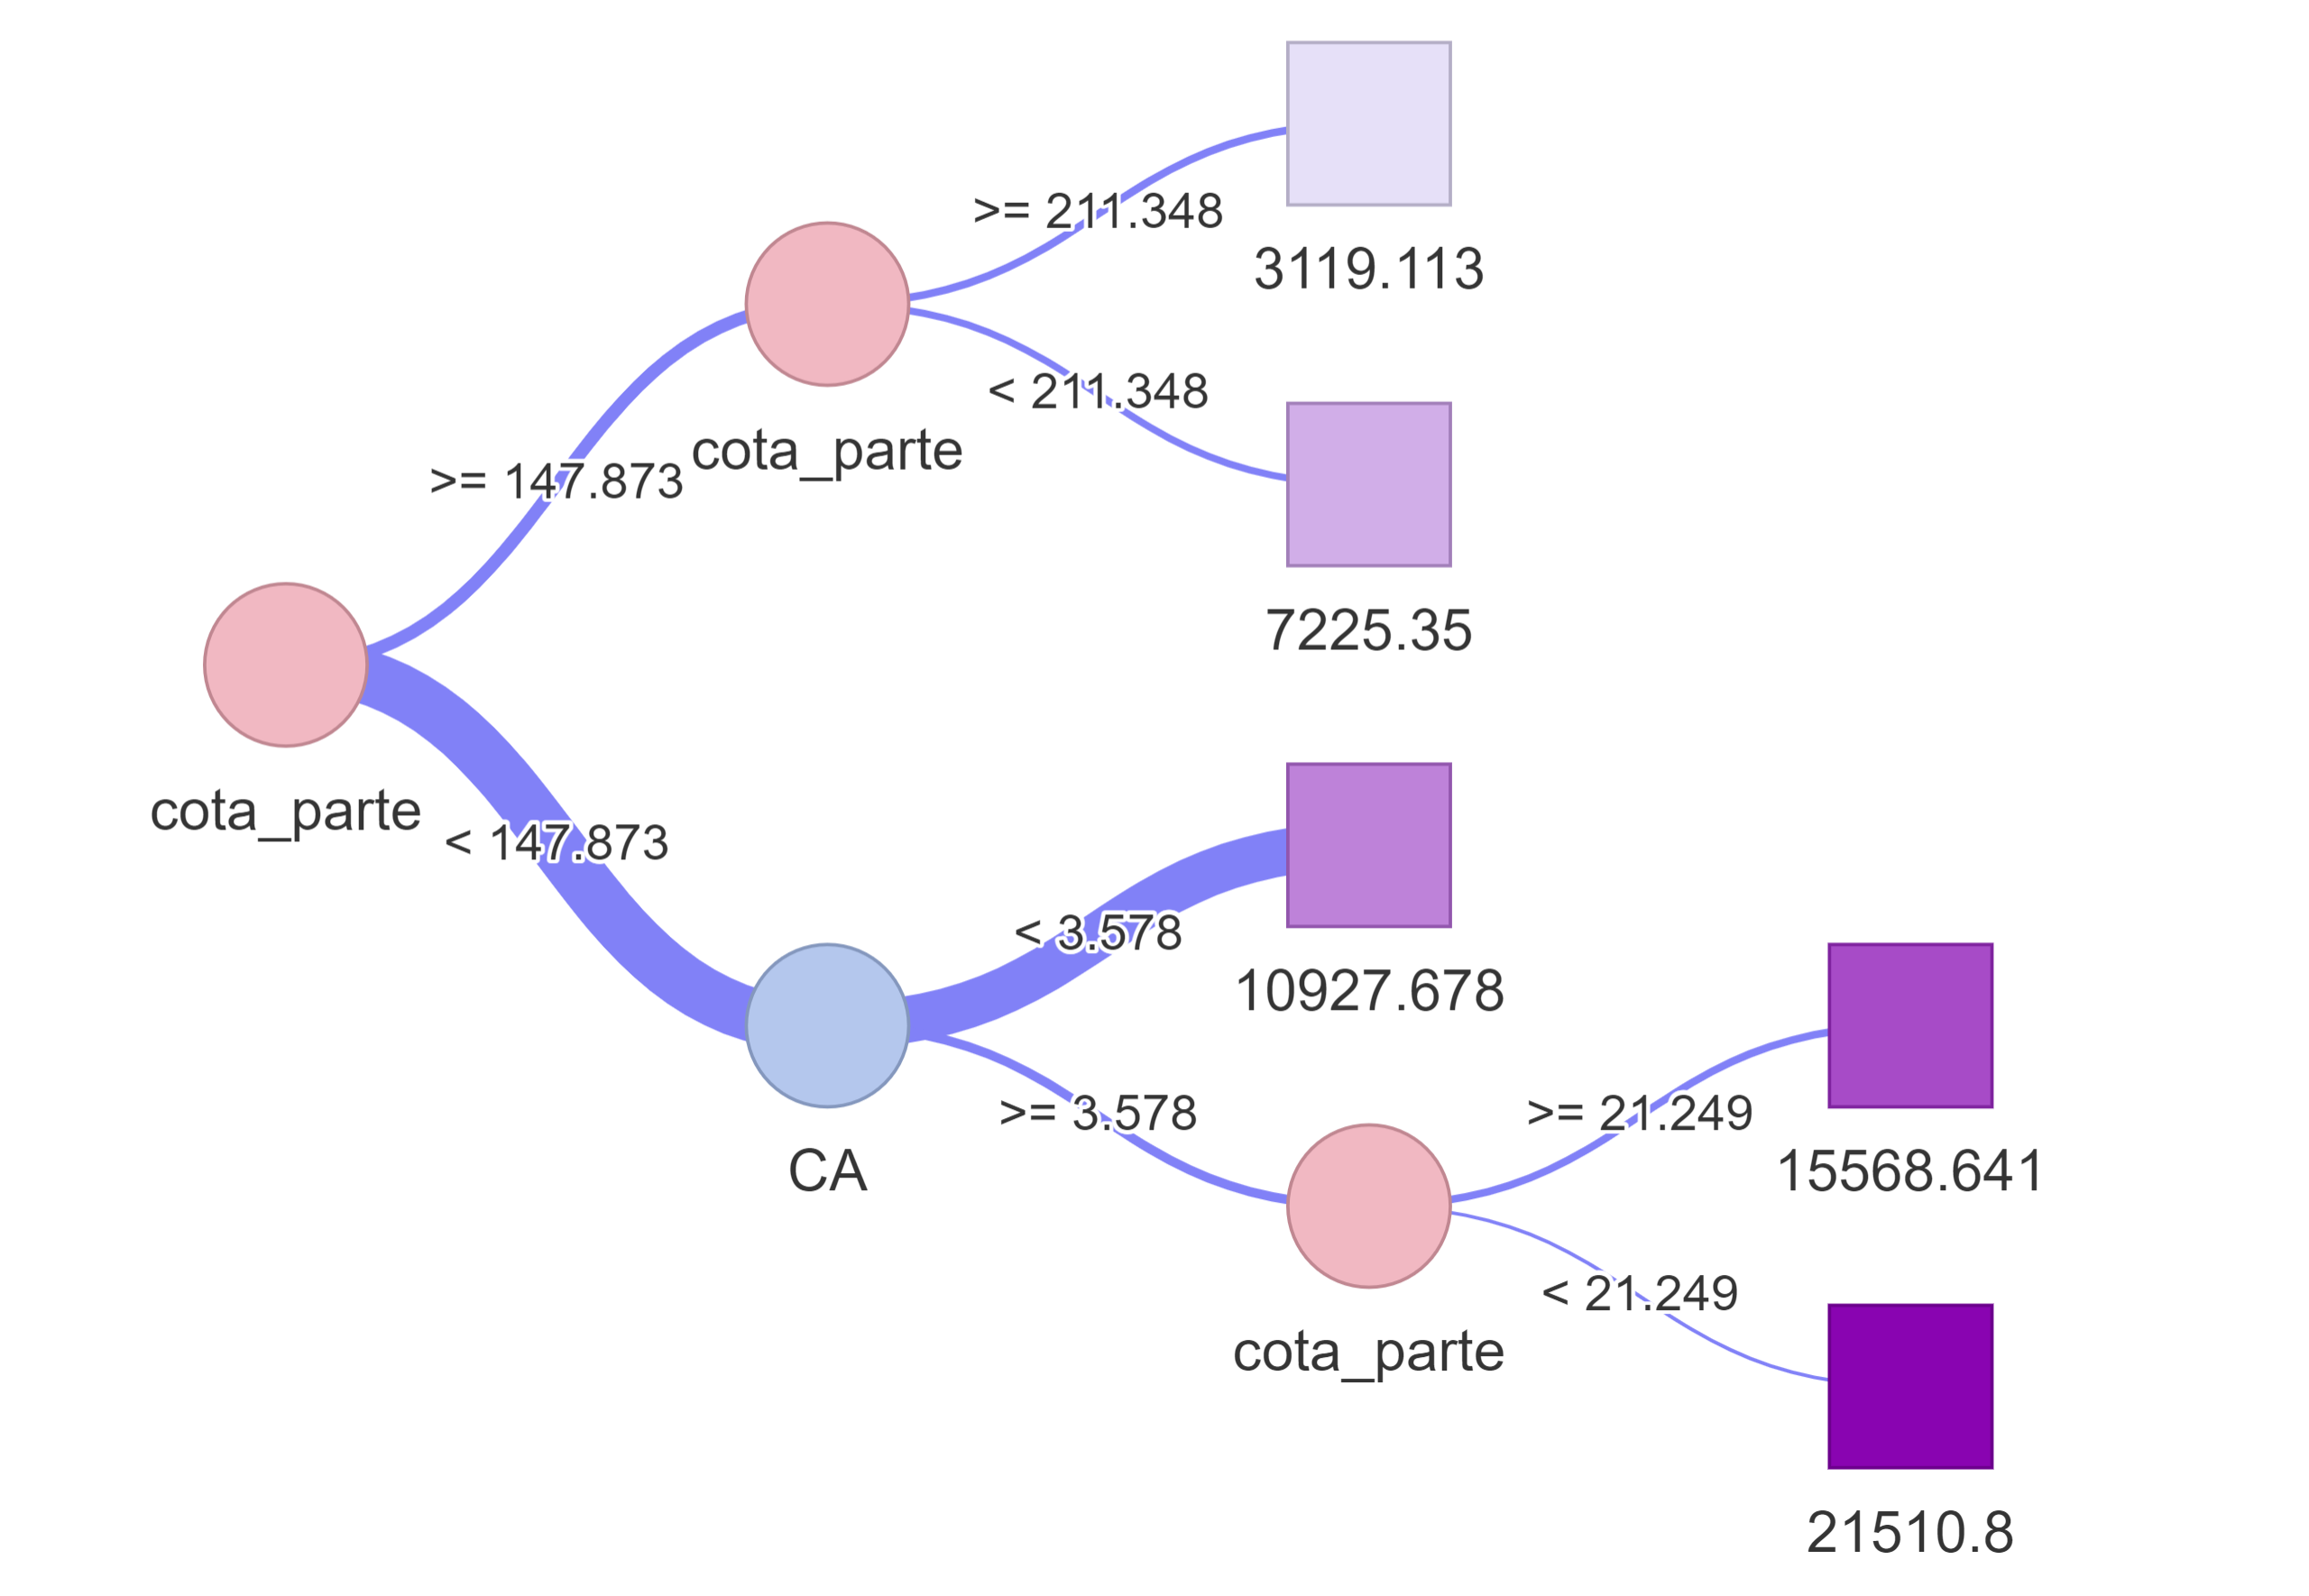
\includegraphics[width = .7\textwidth]{imagens/tree_example.png}
    \end{figure}
\end{frame}

\begin{frame}
    \frametitle{Comparação entre os modelos}

    \begin{table}
        \centering
        \resizebox{.75\textwidth}{!}{%
        \begin{tabular}{rcl}
            Modelo & Variáveis & $R^2$ na base de teste \\
            \hline
            Regressão Linear & (restrita) & 0,239\\
            \textit{Random Forest} & (restrita) & 0,288\\
            \textit{Random Forest} & (irrestrita) & 0,848
        \end{tabular}%
    }
    \end{table}
    
    \vspace{25pt}

    Modelo na versão irrestrita adiciona as variáveis: 
    \begin{itemize}
        \item Número total de unidades
        \item Latitude e longitude do raster
        \item Áreas de terreno, construída e ocupada

    \end{itemize}
\end{frame}

\begin{frame}
    \frametitle{Importância das variáveis do modelo}
    \begin{figure}
        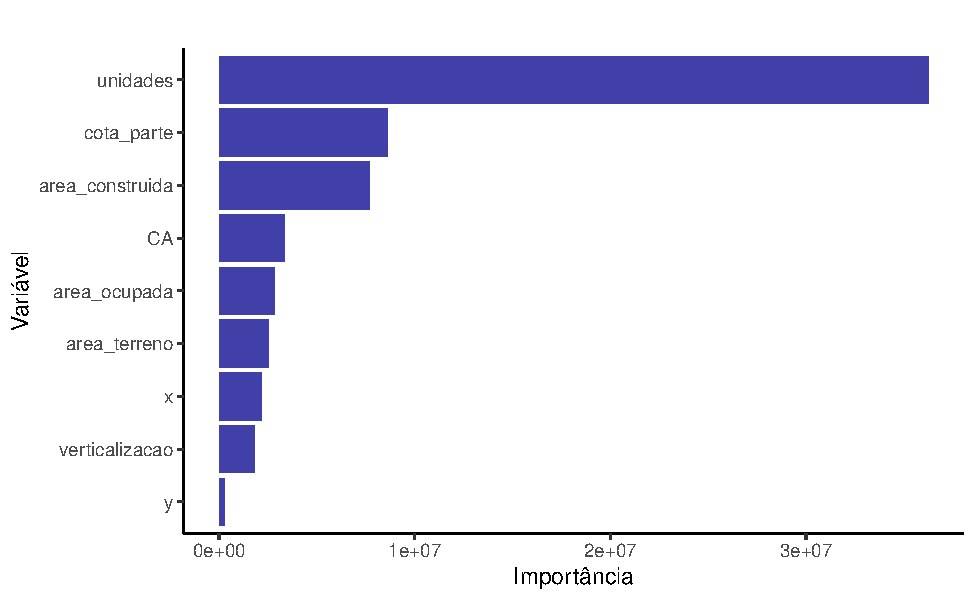
\includegraphics[width = .8\textwidth]{imagens/var_importance.pdf}
    \end{figure}
\end{frame}

\begin{frame}
    \frametitle{Retomando\dots}
    \begin{equation*}
        \frac{\textit{População}_i}{\textcolor{BrickRed}{\textbf{\textit{A. Total}}}_i}
        =\beta_0
        +\beta_1\left(\frac{\textit{A. Construída}_i}{\textit{A. do Terreno}_i}\right)
        +\beta_2\left(\frac{\textit{A. Terreno}_i}{\textit{N. unidades}_i}\right)
        +\beta_3\left(\frac{\textit{A. Construída}_i}{\textit{A. Ocupada}_i}\right)
        +\varepsilon_i
    \end{equation*}

    \vspace{50pt}

    \begin{equation*}
        \text{Área total} = \text{Área de Terreno} + \text{Área não residencial}
    \end{equation*}

\end{frame}

\begin{frame}
    \frametitle{Comparação entre os modelos}
    \centering

    \begin{table}
        \centering
        \caption{Resultados utilizando área total para calcular a densidade}
        \resizebox{.6\textwidth}{!}{%
        \begin{tabular}{rcl}
            Modelo & Variáveis & $R^2$ na base de teste \\
            \hline
            Regressão Linear & (restrita) & 0,239\\
            \textit{Random Forest} & (restrita) & 0,288\\
            \textit{Random Forest} & (irrestrita) & 0,848
        \end{tabular}%
    }
    \end{table}

    \vspace{10pt}

    % \textbf{Resultados utilizando área do terreno}
    \begin{table}
        \centering
        \caption{Resultados utilizando área do terreno para calcular a densidade}
        \resizebox{.6\textwidth}{!}{%
        \begin{tabular}{rcl}
            Modelo & Variáveis & $R^2$ na base de teste \\
            \hline
            Regressão Linear & (restrita) & 0,436\\
            \textit{Random Forest} & (restrita) & 0,727\\
            \textit{Random Forest} & (irrestrita) & 0,796
        \end{tabular}%
    }
    \end{table}
    
    
\end{frame}

\begin{frame}
    \frametitle{Importância das variáveis do modelo}
    \framesubtitle{Cálculo da densidade através da área de terreno}
    \begin{figure}
        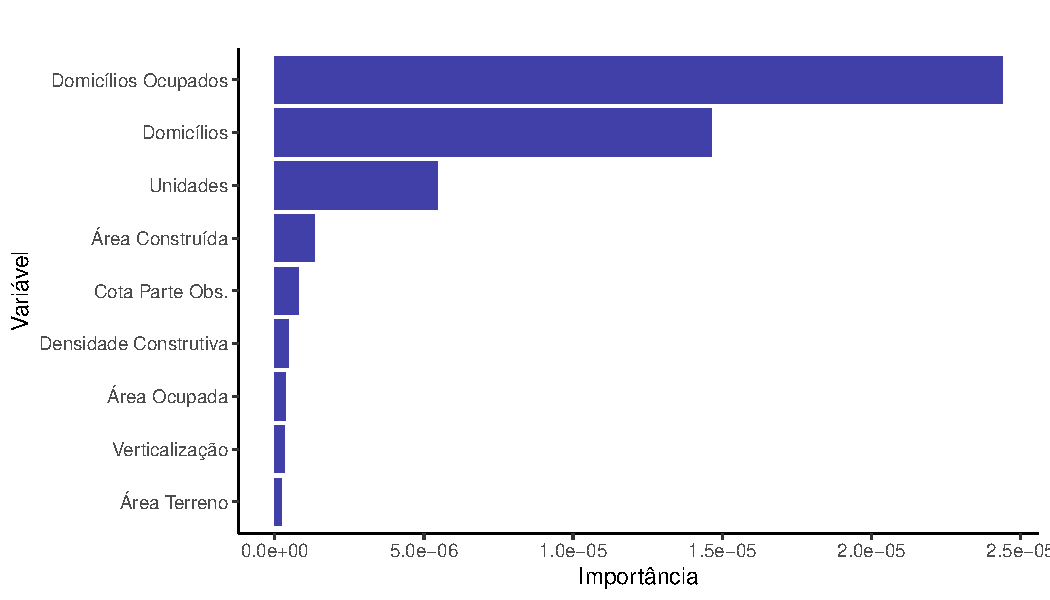
\includegraphics[width = .8\textwidth]{imagens/var_importance_densmod.pdf}
    \end{figure}
\end{frame}


\section{Conclusão}

\begin{frame}
    \frametitle{Conclusão}
    \begin{itemize}
        \item Eficiência dos instrumentos
        \begin{itemize}
            \item Cota parte $>$ CA $>$ pavimentos $=$ 0
        \end{itemize}
        \item Fatores adicionais
        \begin{itemize}
            \item Proximidade ao emprego é um fator importante não considerado
            \item Necessidade de investigar outros fatores em futuras pesquisas
        \end{itemize}
        \item Moradia informal
        \begin{itemize}
            \item 53\% dos domicílios não inscritos no Cadastro Imobiliário Fiscal
            \item Instrumentos impactam no máximo metade da cidade
        \end{itemize}
        \item Adensamento informal
        \begin{itemize}
            \item Regiões informais mostram maior adensamento
            \item Exemplo: favela de Paraisópolis, região mais densa da cidade
        \end{itemize}
    \end{itemize}
\end{frame}

\end{document}
